%% Manuscript draft v0.1 (2026-10-28) -- Elsevier elsarticle, author-year (Biosystems Engineering style).
%% Red [TBD: ...] marks results that are still running (SAM segmentation, closed-loop evaluation) or text to verify.
%% Numbers outside [TBD] come from paper/results/*.json (scripts in paper/experiments/).
\documentclass[preprint,review,12pt,authoryear]{elsarticle}

\usepackage{amsmath,amssymb}
\usepackage{graphicx}
\usepackage{booktabs}
\usepackage{multirow}
\usepackage{xcolor}
\usepackage{algorithm}
\usepackage{algpseudocode}
\usepackage{siunitx}
\usepackage{hyperref}
\usepackage{lineno}
\usepackage{adjustbox}
\linenumbers

\graphicspath{{../../figures/}}
\newcommand{\tbd}[1]{\textcolor{red}{[TBD: #1]}}
\newcommand{\pekm}{PEKM}
\newcommand{\fdm}{SAM-FDM}
\newcommand{\bench}{HarvestMem-Sim}
\sisetup{detect-all}

\journal{Biosystems Engineering}

\begin{document}

\begin{frontmatter}

\title{HarvestMem: event-centric memory for vision--\hspace{0pt}language--\hspace{0pt}action harvesting robots under foliage occlusion}

\author[a]{\tbd{Author 1}}
\author[a]{\tbd{Author 2}}
\author[a]{\tbd{Corresponding author}\corref{cor1}}
\cortext[cor1]{Corresponding author. E-mail: \tbd{email}}
\address[a]{\tbd{Affiliation, city, postcode, country}}

\begin{abstract}
Selective harvesting robots must act on information they can no longer see: wind-blown foliage hides ripe fruits, and harvesting quotas depend on picks whose results lie outside the camera view. Vision--language--action (VLA) policies promise a single instruction-driven controller for such tasks, yet their memory is a fixed number of past frames sampled uniformly in time. We show that this time-indexed memory loses picks at a rate that grows with operating time: its coverage of completed picks decays inversely with elapsed time, and at a 16-frame budget it misses 43\% of them. We propose HarvestMem, an event-centric memory framework that indexes memory by physical interaction events rather than by time. Its spatial memory, built by a SAM-based fruit distance module (SAM-FDM), anchors every fruit in 3D while it is visible. Its episodic memory, Picking-Event Keyframe Memory (PEKM), detects picks from the end-effector-to-fruit distance and reserves memory slots for their contact and detachment keyframes, without extra parameters, tokens or inference cost. On HarvestMem-Sim, a new benchmark with a 7-DoF arm, foliage occlusion and quota counting, PEKM retained 99.6\% of completed picks versus 57.0\% for uniform memory, and with 8 frames outperformed uniform memory with 16. Using only RGB-D images and proprioception, SAM-FDM localized fruits within 0.48~cm, recovered every leaf-hidden ripe fruit and reproduced the ground-truth picking events exactly, whereas anchors built after occlusion left no occluded episode correctly counted. \tbd{one sentence on closed-loop success}
\end{abstract}

\begin{highlights}
\item Fruit harvesting is cast as a fixed-budget memory problem for VLA robots.
\item Uniform memory loses picks at a rate that grows with operating time.
\item Event-indexed memory keeps 99.6\% of picks vs 57.0\%, at zero extra cost.
\item SAM-based 3D fruit anchors recover every leaf-hidden ripe fruit.
\item Spatial memory before occlusion is a precondition for event memory.
\end{highlights}

\begin{keyword}
Selective harvesting \sep Vision--language--action model \sep Temporal memory \sep Keyframe selection \sep Foliage occlusion \sep Segment Anything Model \sep Imitation learning
\end{keyword}

\end{frontmatter}

%% Nomenclature (optional box; Biosystems Engineering encourages it)
\section*{Nomenclature}
\begin{tabular}{lp{11.2cm}}
$B$ & memory budget (number of past frames kept), here $B=16$\\
$c_U(t)$ & coverage of a completed pick by uniform memory at decision time $t$\\
$S_e$, $W$ & key set of event $e$ (frames within $\pm W$ of its contact and release keyframes), $W=3$\\
$d_t$ & distance from the tool centre point (TCP) to the nearest pickable fruit at frame $t$ (m)\\
$k$ & maximum number of event keyframes reserved in the memory\\
$r$, $\mathrm{tol}$ & event radius and contact tolerance (m)\\
$\mathcal{M}_t$ & set of past frames in the memory at decision time $t$\\
$\sigma$, $\tau$ & stationary standard deviation (rad) and correlation time (steps) of the DART-H noise\\
DART & disturbances for augmenting robot trajectories \citep{laskey2017dart}\\
FDM & fruit distance module\\
PEKM & picking-event keyframe memory\\
TCP & tool centre point\\
VLA & vision--language--action (policy)\\
\end{tabular}

\section{Introduction}
\label{sec:intro}

Harvesting is among the most labour-intensive and time-critical operations in fruit production. The shrinking and increasingly expensive seasonal workforce has made robotic selective harvesting a long-standing goal of agricultural engineering \citep{bac2014harvesting,kootstra2021selective,zhou2022intelligent}. Decades of research have produced capable systems for sweet pepper \citep{arad2020sweetpepper}, kiwifruit \citep{williams2019kiwifruit} and apple \citep{silwal2017apple}. Each, however, is a pipeline of detection, localization, planning and grasping modules engineered for one crop, one decision rule and one scene layout, and a new harvesting objective means a new software project. Vision--language--action (VLA) policies offer a different paradigm. A single network, pretrained on web-scale vision--language data and large robot datasets, maps camera images, proprioception and a natural-language instruction directly to actions \citep{brohan2023rt2,kim2024openvla,black2024pi0,pi05_2025}. For agriculture the appeal is fundamental: \emph{which} fruits to pick, \emph{how many} and \emph{where} to put them become an instruction rather than an engineering effort.

\paragraph{Harvesting is a memory problem} A harvesting robot rarely has in its current view the information it needs for its next decision. Three situations, routine in orchards and greenhouses, make this concrete:
\begin{enumerate}
\item \emph{Foliage occlusion.} Leaves moved by wind or by the manipulator hide ripe fruits that were visible moments earlier \citep{hemming2014detectability}. A fruit that cannot be seen must still be picked.
\item \emph{Quota harvesting.} Grading, sampling and selective thinning require a given number of fruits, so the robot must know how many it has already picked.
\item \emph{Out-of-view containers.} The collection bin is usually outside the working camera's field of view, so the outcome of earlier picks cannot be re-observed.
\end{enumerate}
Forgetting has a direct agronomic cost in each case. A forgotten ripe fruit is lost yield and is left to over-mature on the plant. A forgotten pick leads to over-harvesting that violates the quota. A fruit whose ripeness was misjudged ends as unmarketable produce. The problem is not marginal: in the benchmark introduced here, a leaf-hidden ripe fruit is invisible in a median 78\% of the frames in which it still hangs on the tree, so the decision to pick it must be taken largely from memory.

\paragraph{Time-indexed memory forgets more the longer the robot works} Memory-augmented VLA policies keep a bounded number of past frames, because every frame adds visual tokens and the cost of attention grows quadratically with the number of tokens \citep{vaswani2017attention}. The standard way to fill this budget is to sample the history uniformly in time. We show that this design has a structural flaw for manipulation. The frames that define a pick (the gripper closing on a fruit, the fruit detaching from its stem) span only about a dozen frames, and fewer than 5\% of uniformly sampled memory frames show the gripper within 3~cm of a fruit to be picked. With $B$ frames spread evenly over $t$ elapsed frames, a pick is retained with a probability of roughly $(B-1)|S|/t$, where $|S|$ is the length of its key window. Coverage therefore decays inversely with operating time (Section~\ref{sec:coverage}). The measurements confirm this prediction. At a 16-frame budget, uniform memory misses 43\% of completed picks, can recover the pick count at only 43\% of decisions, and, after 600 frames of operation, loses even the \emph{most recent} pick at 78\% of decisions. These losses are consequential for the policy. On a general manipulation-memory benchmark, removing the memory of the same base VLA reduces success from 66.7\% to 1.7\%, and halving its budget from 32 to 16 frames reduces success from 64.4\% to 26.7\% (Section~\ref{sec:res_general}). What a VLA remembers is a first-order determinant of what it can do.

\paragraph{Why the obvious remedies fall short} \emph{Enlarging the memory} treats the symptom: to keep events, a uniform budget must grow linearly with operating time, and the cost of attention grows quadratically with the budget, which embedded field computers cannot afford. \emph{Better per-frame perception} cannot see what is hidden. A detector without memory loses a fruit as soon as leaves cover it and mistakes a carried fruit for a new target. In our experiments, per-frame detection recovers the correct pick count in only 62\% of episodes. \emph{Learned memory selection or token compression} adds parameters and training signals, may behave differently in training and deployment, and makes it hard to audit what the robot remembered when it failed. What is missing is a \emph{principle} that tells a harvesting robot what is worth remembering.

\paragraph{Key insight: index memory by events, not by time} Our central observation is that in agricultural manipulation, task-relevant information is not spread uniformly over time. It is concentrated at a few physical interaction events. Every pick consists of an approach, a contact and a detachment, and these moments change the state of the task: a fruit leaves the plant and the count increments. They are also physically observable, because the distance between the tool and the nearest fruit still to be picked drops below the fruit radius at contact and jumps at detachment. This mirrors how people remember activity. Humans segment continuous experience into discrete events and preferentially encode event boundaries \citep{zacks2007event}, and episodic memory binds \emph{what} happened to \emph{where} and \emph{when} it happened \citep{tulving1972episodic,clayton1998episodic}. We carry this structure into robot memory.

\paragraph{HarvestMem: event-centric spatial--episodic memory} We introduce \emph{HarvestMem}, a framework that equips a VLA harvesting policy with two complementary memories coupled through one physical signal (Fig.~\ref{fig:overview}).
\begin{itemize}
\item \textbf{Spatial memory} answers \emph{where} the fruits are. A SAM-based fruit distance module (\fdm) segments fruits with the Segment Anything Model \citep{kirillov2023sam} while they are visible and anchors each one in 3D. The anchors persist when foliage hides the fruit and are retired when the fruit is picked.
\item \textbf{Episodic memory} answers \emph{what} happened and \emph{when}. Picking-Event Keyframe Memory (\pekm) detects picks causally from the distance between the tool and the nearest anchored fruit, and reserves slots in the VLA's fixed memory for their contact and detachment keyframes.
\end{itemize}
The design changes \emph{what} the policy remembers, not \emph{how much} or \emph{how}. \pekm\ adds no parameters, no tokens and no inference cost. It contains the base model's uniform memory as the special case $k=0$, and it is applied identically in training and deployment. Because perception and memory communicate only through a scalar distance, the detector can be replaced without retraining the policy, and every memory the policy saw can be reproduced from a logged signal. Phase-aware recovery demonstrations (DART-H) complement the memory by addressing the compounding errors of closed-loop imitation \citep{ross2011dagger}.

\paragraph{Contributions} The main contributions of this work are:
\begin{enumerate}
\item \textbf{Problem formulation and benchmark.} We formulate selective harvesting with a VLA policy as a fixed-budget memory-allocation problem. We release \bench, a procedural ManiSkill3 orchard with a commercial 7-DoF RealMan RM75-B arm and two tasks that cannot be solved from the current view: picking leaf-hidden ripe fruits (FruitOccludedRipe) and meeting a quota with an out-of-view basket (FruitCount). The benchmark includes per-frame ground truth for events, occlusion and perception.
\item \textbf{Event-centric memory with a coverage analysis.} We identify a structural limitation of time-indexed memory: its coverage of interaction events decays inversely with operating time. A simple sampling model predicts the measured coverage to within 0.012. We propose \pekm, which guarantees coverage of the most recent picks independently of episode length. It retains 99.6\% of completed picks against 57.0\% for uniform memory at the same budget, and with 8 frames it outperforms uniform memory with 16, at zero additional cost.
\item \textbf{Spatial--episodic coupling through promptable segmentation.} \fdm\ turns RGB-D images and proprioception into 3D fruit anchors, using visual (depth vacancy) and proprioceptive (grasp) evidence of picking, and reproduces the ground-truth picking events exactly. Its ablations establish that spatial memory acquired before occlusion is a \emph{precondition} for episodic memory: when anchors are built after occlusion, the occluded-task count accuracy falls from 1.00 to 0.00. A robustness analysis turns event memory into an explicit accuracy specification for perception modules.
\item \textbf{Phase-aware recovery demonstrations (DART-H).} Temporally correlated joint noise is injected only in free-motion phases, while clean planner actions are recorded as labels. This targets the covariate shift that limits closed-loop imitation in harvesting.
\item \textbf{A rigorous evaluation protocol.} Evaluation follows a protocol sealed before the formal runs. It uses paired bootstrap with Holm correction and equivalence margins, and audits at every decision that the frames fed to the model match the declared selection rule. Counterfactual controls separate the effect of event information from the mere perturbation of changing frames.
\end{enumerate}

The remainder of the paper is organized as follows. Section~\ref{sec:related} positions the work. Section~\ref{sec:benchmark} describes \bench. Section~\ref{sec:method} presents HarvestMem: the coverage analysis, \pekm, \fdm\ and DART-H. Section~\ref{sec:design} details the experimental design and Section~\ref{sec:results} reports the results. Section~\ref{sec:discussion} discusses implications and limitations for agricultural deployment, and Section~\ref{sec:conclusions} concludes.

\begin{figure}[t]
\centering
\fbox{\parbox{0.92\linewidth}{\centering\vspace{2.2cm}\tbd{Fig.~1 (to be drawn). Left: the two memory needs of harvesting, a ripe fruit hidden by wind-blown leaves and a quota with an out-of-view basket. Middle: time-indexed (uniform) memory misses the short pick events. Right: HarvestMem, with spatial memory (3D fruit anchors from SAM, \emph{where}) and episodic memory (contact/detachment keyframes from PEKM, \emph{what} and \emph{when}) coupled by the tool-to-fruit distance $d_t$ and feeding the VLA.}\vspace{2.2cm}}}
\caption{HarvestMem in a nutshell. Harvesting requires remembering fruits that are no longer visible and picks whose results are out of view. Instead of sampling memory uniformly in time, HarvestMem indexes it by physical events: fruits are anchored in 3D while visible (spatial memory), and the contact and detachment keyframes of picks are reserved in the VLA's fixed memory budget (episodic memory).}
\label{fig:overview}
\end{figure}

\section{Related work}
\label{sec:related}

\subsection{Harvesting robots and fruit perception}
Reviews of harvesting robotics identify fruit detection under occlusion, localization accuracy and cycle time as the main bottlenecks \citep{bac2014harvesting,kootstra2021selective,zhou2022intelligent}. Field systems for sweet pepper \citep{arad2020sweetpepper}, kiwifruit \citep{williams2019kiwifruit} and apple \citep{silwal2017apple} follow a detect--localize--plan--grasp pipeline. Deep learning has replaced hand-crafted colour and shape features for fruit detection and segmentation \citep{sa2016deepfruits,kamilaris2018survey,koirala2019review}. Typical models are instance segmentation networks such as Mask R-CNN \citep{he2017maskrcnn} and single-stage detectors of the YOLO family \citep{redmon2016yolo}, often combined with depth or multi-view geometry for 3D localization \citep{gene2020fruit,kang2020apple}. Promptable foundation models for segmentation, Segment Anything (SAM) and SAM~2 \citep{kirillov2023sam,ravi2024sam2}, enable zero-shot masks from point or box prompts, and their use in agriculture is growing \tbd{cite 2--3 verified agricultural SAM applications}. Our \fdm\ uses SAM in this promptable mode, but its output is not a detection map for a planner. It is a scalar distance signal that organizes the memory of a learned policy.

\subsection{Occlusion and active perception in harvesting}
Occlusion by leaves and branches is a primary cause of missed fruits; detectability depends strongly on viewpoint \citep{hemming2014detectability}. Proposed remedies include multiple or moving cameras, next-best-view planning and active manipulation of foliage \tbd{cite verified works on multi-view / next-best-view / leaf pushing for harvesting}. These methods address what is not visible in the \emph{current} view. They rarely address fruits that were seen earlier and are hidden now, which calls for temporal or spatial memory rather than a better viewpoint. \bench\ isolates exactly this case: every leaf-hidden ripe fruit is fully visible before the gust.

\subsection{Vision--language--action policies and imitation learning}
VLA models extend vision--language models with action outputs: RT-2 \citep{brohan2023rt2}, OpenVLA \citep{kim2024openvla}, Octo \citep{octo2024}, and the flow-matching policies $\pi_0$ and $\pi_{0.5}$ \citep{black2024pi0,pi05_2025}, which build on PaliGemma \citep{beyer2024paligemma}, SigLIP \citep{zhai2023siglip} and flow matching \citep{lipman2023flow}. Policies trained from demonstrations, including Diffusion Policy \citep{chi2023diffusion} and ACT \citep{zhao2023act}, suffer from covariate shift. Small errors drive the robot into states absent from the demonstrations, where errors compound \citep{ross2011dagger}. Interactive corrections (DAgger) or noise injection during demonstration (DART, \citealp{laskey2017dart}) are the standard remedies. DART-H follows the latter, which needs no expert in the loop, and adapts it to the phase structure of harvesting. Applications of VLA policies to agricultural manipulation are still rare \tbd{cite verified early agricultural VLA / foundation-model robotics works, if any}.

\subsection{Memory and keyframes in robot policies}
Long-horizon manipulation benchmarks show that policies without history fail on tasks that require recalling past observations \tbd{cite RoboMME / memory benchmarks (verify)}. Memory-augmented VLAs keep a bounded history of visual tokens \tbd{cite MME-VLA / memory-as-modulator base model (verify)}. Keyframes are widely used in manipulation for other purposes: as action targets in keyframe-based policies \citep{shridhar2022peract} and as waypoints that compress demonstrations \citep{shi2023awe}. In video understanding, memory banks and keyframe selection compress long videos for multimodal models \citep{he2024malmm}. Cognitive science suggests that people segment continuous activity into discrete events and remember event boundaries preferentially \citep{zacks2007event}. To our knowledge, no prior work selects the memory frames of a VLA policy from task-defined physical events, nor studies memory selection for agricultural manipulation.

\subsection{Positioning of this work}
Table~\ref{tab:positioning} contrasts the memory designs available to a VLA policy under a fixed budget. Time-indexed designs keep either the recent past (a sliding window) or the whole past at a resolution that falls with elapsed time (uniform sampling), so short interaction events are kept only by chance. Learned memory banks and token compression can in principle discover what matters. They do so, however, implicitly, with additional parameters and training signals, and their selections are hard to audit. HarvestMem differs in three ways:
\begin{enumerate}
\item The unit of memory is a \emph{physical interaction event} defined by task geometry, not a time slot or a learned feature.
\item Selection is a parameter-free deterministic function that is identical in training and deployment and contains uniform memory as a special case.
\item Episodic memory of events is coupled to an explicit \emph{spatial} memory of objects acquired before occlusion. The ablations of Section~\ref{sec:res_chain} show that this coupling is necessary rather than optional.
\end{enumerate}

\begin{table}[t]
\centering
\caption{Memory designs for a VLA policy under a fixed budget. $\checkmark$: yes; $\times$: no; $\circ$: only by chance or implicitly.}
\label{tab:positioning}
\footnotesize
\begin{adjustbox}{max width=\textwidth}\begin{tabular}{lcccccc}
\toprule
Memory design & Distant past & Pick events kept & Fixed cost & No extra params & Train = deploy & Physically grounded\\
\midrule
No memory (current frame) & $\times$ & $\times$ & $\checkmark$ & $\checkmark$ & $\checkmark$ & $\times$\\
Recent window & $\times$ & $\circ$ & $\checkmark$ & $\checkmark$ & $\checkmark$ & $\times$\\
Uniform sampling (base model) & $\checkmark$ & $\circ$ & $\checkmark$ & $\checkmark$ & $\checkmark$ & $\times$\\
Learned memory bank / compression & $\checkmark$ & $\circ$ & $\checkmark$ & $\times$ & $\checkmark$ & $\times$\\
\textbf{PEKM (HarvestMem)} & $\checkmark$ & $\checkmark$ & $\checkmark$ & $\checkmark$ & $\checkmark$ & $\checkmark$\\
\bottomrule
\end{tabular}\end{adjustbox}
\end{table}

\section{\bench: a memory-dependent harvesting benchmark}
\label{sec:benchmark}

\subsection{Procedural orchard scene}
\bench\ is built on ManiSkill3 \citep{tao2025maniskill3} (environment \texttt{FruitPick-v1}). Each episode samples a tree with a trunk, branches and leaf clusters, and 4--6 spherical fruits of radius 2.5--2.9~cm. Fruits hang at heights of 0.44--0.64~m, at distances of 0.38--0.50~m from the robot base and within $\pm 28^\circ$ of azimuth. The layout sampler guarantees that each fruit has a horizontal-approach inverse-kinematics solution, that no branch blocks its approach corridor, and that fruits do not occlude each other in the front camera. A fruit is kinematically attached to its stem until it has been held between both fingers for two consecutive control steps; it then becomes a dynamic rigid body. Training, validation and test seeds are drawn from disjoint ranges.

\subsection{Robot and sensing}
The robot is a RealMan RM75-B 7-DoF arm with an EG2 parallel gripper under joint-position control (a 6-DoF RM65-B is also supported). Observations are a front camera and a wrist camera (both RGB-D, $256\times256$ pixels; the front camera has a $55^\circ$ field of view) and an 8-dimensional state (seven joint angles and one finger position). Actions are seven absolute joint targets and a gripper command.

\subsection{Tasks}
\label{sec:tasks}
Figure~\ref{fig:scene} shows both tasks.
\begin{itemize}
\item \textbf{FruitOccludedRipe.} Red (ripe) and green (unripe) fruits hang together. During a 30-step observation phase, a gust between steps 8 and 20 blows two leaf clusters in front of two fruits, at least one of them ripe, so ``hidden'' does not imply ``ripe''. The instruction is to put all ripe fruits into the basket. Leaves are pushed aside when the gripper comes within 15~cm, so the final approach is visible, but \emph{finding} a hidden ripe fruit requires remembering it. Success: every ripe fruit in the basket and no unripe fruit in it. Failure: an unripe fruit in the basket or a fruit dropped.
\item \textbf{FruitCount.} All $M$ fruits are ripe, and the instruction asks for exactly $N<M$ of them, with $N$ varying per episode (2--5). The basket is outside the front camera view, so the policy can only know how many it has picked by remembering its own picks. Success: exactly $N$ fruits in the basket. Failure: more than $N$ in the basket or a fruit dropped.
\end{itemize}

\begin{figure}[t]
\centering
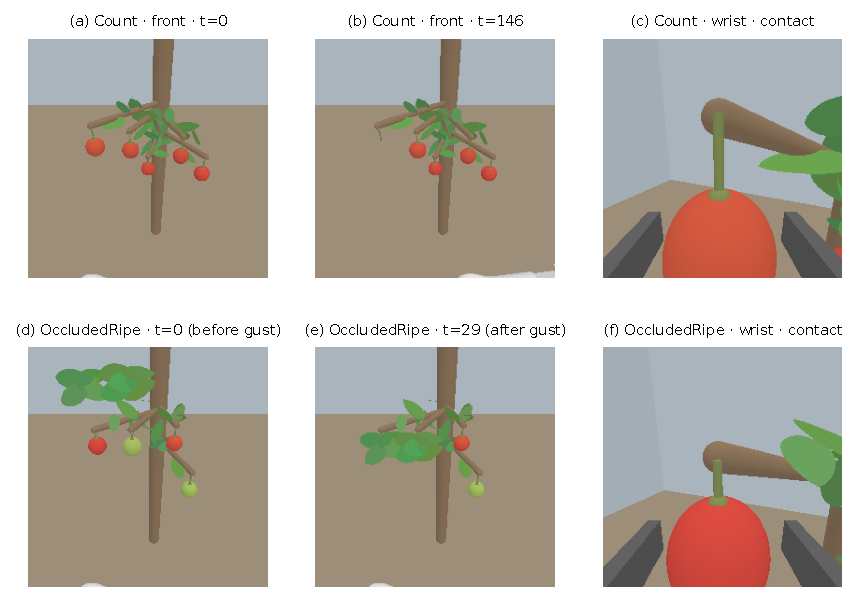
\includegraphics[width=\linewidth]{fig2_scene}
\caption{\bench\ tasks. (a--c) FruitCount: front view at the start and after one pick, and the wrist view at contact. (d--f) FruitOccludedRipe: the front view before and after the wind gust (two leaf clusters now hide fruits) and the wrist view at contact.}
\label{fig:scene}
\end{figure}

\subsection{Demonstrations}
A scripted demonstrator plans with mplib \citep{mplib} through eight phases: observe, reach, approach, grasp, pull, carry, release and settle. An attempt that fails (planning failure, no detachment, missed basket, task not completed) is discarded and the seed is advanced, so only successful demonstrations are kept. Every frame stores the simulator ground truth: fruit poses and attachment, visible pixel counts per camera, phase labels and the TCP pose. Recovery demonstrations (DART-H, Section~\ref{sec:dart}) use the same demonstrator with execution noise.

Table~\ref{tab:dataset} summarizes the 640 demonstrations: 200 clean training, 200 DART-H training, 40 development (used only for a go/no-go gate) and 200 validation episodes. Table~\ref{tab:occlusion} quantifies occlusion. After the gust, the targeted fruits are fully invisible in the front camera. Over all frames in which an occluded fruit is still on the tree, it is invisible in 72\% of frames on average (median 78\%). Remembering where it is, rather than seeing it, is therefore a precondition for picking it.

\begin{table}[t]
\centering
\caption{Benchmark statistics (mean $\pm$ SD [min, max]). Acceptance: fraction of demonstrator attempts that succeeded.}
\label{tab:dataset}
\small
\begin{adjustbox}{max width=\textwidth}\begin{tabular}{llrcccc}
\toprule
Set (episodes) & Task & $n$ & Steps & Fruits & Picks & Acceptance\\
\midrule
Clean train (0--99) & FruitCount & 100 & $474\pm124$ [320, 757] & 4.73 & 2.85 & 0.96\\
 & FruitOccludedRipe & 100 & $412\pm85$ [295, 710] & 4.69 & 2.54 & 0.98\\
DART-H train (100--199) & FruitCount & 100 & $455\pm133$ [314, 876] & 4.62 & 2.70 & 0.57\\
 & FruitOccludedRipe & 100 & $397\pm89$ [297, 672] & 4.78 & 2.46 & 0.66\\
Development (200--219) & FruitCount & 20 & $487\pm162$ [321, 766] & 5.05 & 3.10 & 1.00\\
 & FruitOccludedRipe & 20 & $369\pm71$ [300, 471] & 4.60 & 2.35 & 0.95\\
Validation (0--49) & FruitCount & 50 & $459\pm142$ [314, 904] & 4.58 & 2.82 & 0.98\\
 & FruitOccludedRipe & 50 & $396\pm87$ [300, 630] & 4.72 & 2.50 & 0.96\\
Validation (50--99) & FruitCount & 50 & $499\pm169$ [322, 1037]$^{a}$ & 4.67 & 2.98 & 0.91\\
 & FruitOccludedRipe & 50 & $392\pm73$ [304, 534] & 4.54 & 2.52 & 0.98\\
\bottomrule
\end{tabular}\end{adjustbox}

\footnotesize $^{a}$Statistics over 49 episodes; the ground-truth file of one episode was regenerated after these statistics were computed. Training features: 88,607 samples (clean) and 173,791 samples (clean + DART-H).
\end{table}

\begin{table}[t]
\centering
\caption{Occlusion and phase structure (clean training set).}
\label{tab:occlusion}
\small
\begin{adjustbox}{max width=\textwidth}\begin{tabular}{lc}
\toprule
Quantity & Value\\
\midrule
Leaf clusters per FruitOccludedRipe episode & 2 (66\% hide a ripe fruit)\\
Occluded fruits fully invisible in the front camera after the gust & 100\%\\
Frames (fruit still on tree) in which an occluded fruit is invisible & mean 72\%, median 78\%\\
Visible fraction of non-occluded fruits after the gust (median) & 1.00\\
Ripe / unripe fruits per FruitOccludedRipe episode & 2.54 / 2.15\\
Mean steps per phase, FruitCount (observe / reach / approach / grasp / & 30 / 118 / 59 / 29 /\\
\quad pull / carry / release / settle) & 58 / 117 / 23 / 34\\
\bottomrule
\end{tabular}\end{adjustbox}
\end{table}

\section{HarvestMem: event-centric memory for harvesting}
\label{sec:method}

\subsection{Overview and design principles}
\label{sec:principles}
HarvestMem rests on four design principles:
\begin{enumerate}
\item[P1] \textbf{Index memory by events, not by time.} Memory slots go to the moments that change the state of the task, the contact and detachment of each pick, because time-indexed memory provably loses them as operation lengthens (Section~\ref{sec:coverage}).
\item[P2] \textbf{Ground events in physics, not in learned features.} Events are defined by the distance between the tool and the nearest fruit still to be picked. The signal is measurable on a real robot, interpretable, and transferable across crops through a single parameter commensurate with fruit size.
\item[P3] \textbf{Change what is remembered, not how much or how.} The memory budget, token count, architecture and inference cost of the base VLA are unchanged, and the same selection function is used in training and deployment.
\item[P4] \textbf{Remember where before remembering what.} An event on a fruit that foliage hides can be recognized only if the fruit was anchored while visible. Spatial memory is therefore built first and drives episodic memory.
\end{enumerate}
Figure~\ref{fig:system} shows how these principles become a system:
\begin{itemize}
\item \fdm\ (Section~\ref{sec:fdm}) builds the spatial memory, 3D anchors of the fruits, and converts it into a scalar signal $d_t$: the distance from the TCP to the nearest fruit that is still to be picked.
\item A causal detector (Section~\ref{sec:events}) finds picking events in $d_0,\dots,d_t$.
\item \pekm\ (Section~\ref{sec:pekm}) builds the episodic memory by choosing which $B$ past frames the VLA sees.
\item The policy is fine-tuned on demonstrations that include phase-aware recovery data (DART-H, Section~\ref{sec:dart}).
\end{itemize}

\begin{figure}[t]
\centering
\fbox{\parbox{0.92\linewidth}{\centering\vspace{2cm}\tbd{Fig.~3 (to be drawn): system diagram. Front/wrist RGB-D $\rightarrow$ SAM-FDM (colour prompts, SAM masks, 3D anchors, vacancy + grasp evidence) $\rightarrow$ $d_t$ $\rightarrow$ causal event detector $\rightarrow$ PEKM selection $\mathcal{M}_t$ $\rightarrow$ memory expert of the VLA $\rightarrow$ action chunk. Dashed: the same selection function computes the memory of every training sample.}\vspace{2cm}}}
\caption{HarvestMem system. Spatial memory (fruit anchors) and episodic memory (event keyframes) are coupled through the scalar distance $d_t$, the only interface between perception and the policy; $d_t$ selects frame indices and never enters the network.}
\label{fig:system}
\end{figure}

\subsection{Problem formulation}
\label{sec:formulation}
We treat harvesting as a partially observable control problem. At decision time $t$, the policy $\pi_\theta$ receives the current front and wrist images $o_t$, the proprioceptive state $s_t$, the language instruction $l$ and a memory $\mathcal{M}_t$ of past frames, and outputs an action chunk
\begin{equation}
A_t = (a_t,\dots,a_{t+H-1}) = \pi_\theta(o_t, s_t, l, \mathcal{M}_t),\qquad H=20,
\end{equation}
of which the first 16 actions are executed before the next decision. The memory is the output of a selection function
\begin{equation}
\mathcal{M}_t = S\big(\{0,\dots,t\};\, d_{0:t}\big),\qquad |\mathcal{M}_t| = \min(B, t+1),
\label{eq:selection}
\end{equation}
subject to two constraints. The selection is \emph{causal}: it uses only information up to $t$. It is also \emph{budget-preserving}: it returns exactly $B$ frames, the same number as uniform sampling. Under these constraints the only question is \emph{which} frames to keep, so any difference in behaviour can be attributed to memory content rather than memory size.

\subsection{Base policy}
The base policy is a memory-augmented VLA (MME-VLA, \tbd{cite base model}) in the $\pi_{0.5}$ family \citep{pi05_2025}. It has a PaliGemma vision--language backbone (Gemma-2B, \citealp{beyer2024paligemma}), a 300M-parameter action expert that generates action chunks by flow matching \citep{lipman2023flow}, and a 150M-parameter memory expert. Past frames are encoded by the frozen SigLIP encoder \citep{zhai2023siglip} and represented by 16 tokens per frame. The memory expert attends over the $B=16$ selected frames and modulates action generation. We initialize from a checkpoint trained on a general manipulation-memory benchmark (\tbd{cite RoboMME}) and fine-tune all non-vision parameters on \bench. \pekm\ changes only the indices of the frames that enter the memory, so the architecture, the number of tokens and the inference cost are identical across memory conditions.

\subsection{Event signal}
\label{sec:signal}
We define the event signal as
\begin{equation}
d_t = \min_{j \in \mathcal{P}_t} \lVert p^{\mathrm{TCP}}_t - c_j \rVert_2,
\label{eq:signal}
\end{equation}
where $p^{\mathrm{TCP}}_t$ is the TCP position from forward kinematics and $c_j$ is the centre of fruit $j$. $\mathcal{P}_t$ is the set of fruits that are \emph{pickable and still attached} at time $t$: all fruits in FruitCount, ripe fruits in FruitOccludedRipe. If $\mathcal{P}_t$ is empty, $d_t = 10$~m, meaning ``far'' rather than ``unknown''. A frame without a measurement is marked unknown ($d_t = \mathrm{NaN}$). The signal has a clear physical reading. It falls below the fruit radius when the gripper encloses a fruit, and it jumps to the next fruit's distance at the instant the fruit detaches, because a detached fruit is no longer in $\mathcal{P}_t$. During training $d_t$ is computed from the simulator state. At deployment it is produced by \fdm\ with the same definition (Section~\ref{sec:fdm}).

\subsection{Causal picking-event detection}
\label{sec:events}
A frame is \emph{near} if $d_t \le r$ and \emph{far} if $d_t > r$. An unknown frame inherits the state of the last known frame, so a dropped measurement neither starts nor ends an event. An \emph{event} is a maximal run of near frames $[t_s, t_e]$. It contributes two keyframes:
\begin{align}
t^{\mathrm{c}} &= \min\Big\{ f \in [t_s, \min(t_e, t)] : d_f \le \min_{t_s \le g \le \min(t_e,t)} d_g + \mathrm{tol} \Big\}, \label{eq:contact}\\
t^{\mathrm{r}} &= t_e + 1 \quad \text{(only if } t_e < t\text{)}. \label{eq:release}
\end{align}
The contact keyframe $t^{\mathrm{c}}$ is the first frame whose distance is within $\mathrm{tol}$ of the minimum of the run observed so far, i.e.\ the moment the gripper settles around the fruit. The release keyframe $t^{\mathrm{r}}$ is the first far frame after the run, i.e.\ the detachment. Both are computed from frames up to $t$ only. While a run is ongoing it has a contact keyframe but no release keyframe. We use $r=3$~cm and $\mathrm{tol}=5$~mm, chosen on the training set (Section~\ref{sec:res_events}). The radius is commensurate with the fruit radius (2.5--2.9~cm) and below half the inter-fruit spacing.

For noisy deployment signals we also use a \emph{hysteresis} variant. An event is entered when $d_t \le r$ and left only when $d_t > 1.5r$, and runs shorter than 3 frames are discarded. This suppresses spurious events caused by noise around the threshold without the delay of a median filter.

\subsection{Why time-indexed memory loses events: a coverage analysis}
\label{sec:coverage}
Let the key set $S_e$ of a completed pick $e$ be the frames within $\pm W$ of its contact and release keyframes, so that $|S_e| \le 2(2W+1)$. A pick is \emph{covered} at decision time $t$ if the memory holds at least one frame of $S_e$. Uniform memory keeps $B$ frames evenly spaced over $0,\dots,t$, i.e.\ one frame every $\Delta_t = t/(B-1)$ frames. If the phase of this sampling grid is independent of the timing of the pick, the expected number of memory frames in $S_e$ is $|S_e|/\Delta_t$. When $\Delta_t$ is larger than each keyframe window, at most one memory frame falls in each window, and the probability of coverage is approximately
\begin{equation}
c_U(t) \approx \min\!\Big(1,\; \frac{(B-1)\,|S_e|}{t}\Big).
\label{eq:coverage}
\end{equation}
Equation~(\ref{eq:coverage}) has two consequences that are central to harvesting.
\begin{enumerate}
\item \textbf{Forgetting grows with operating time.} For a fixed budget, coverage decays as $1/t$: the longer the robot works, the larger the fraction of its own picks it cannot see in memory. The most recent pick enjoys no protection.
\item \textbf{Budgets must grow linearly with time.} To keep coverage $c$, uniform memory needs $B \ge 1 + c\,t/|S_e|$. With $W=3$ ($|S_e|=14$) and $t=600$ frames, full coverage would require about 44 frames, nearly three times the base model's budget, and the cost of attention grows quadratically with it.
\end{enumerate}
Event indexing removes the dependence on $t$. With keyframe cap $k$, \pekm\ (below) covers the $\lfloor k/2\rfloor$ most recent picks with probability one at every decision time, using a constant two slots per remembered pick. Section~\ref{sec:res_memory} shows that Eq.~(\ref{eq:coverage}) predicts the measured coverage of uniform memory to within 0.012 at every budget, and that \pekm\ keeps the most recent pick at all decision times.

\subsection{Picking-Event Keyframe Memory}
\label{sec:pekm}
Algorithm~\ref{alg:pekm} gives the selection rule. If the episode is shorter than the budget, all frames are kept. Otherwise, keyframes are taken from the most recent event backwards, contact before release, until at most $k$ keyframes are reserved. The remaining $B-|\mathcal{K}|$ slots are filled by frames at evenly spaced positions among the non-key frames 0 to $t$, including the first and the last.

\begin{algorithm}[t]
\caption{PEKM selection at decision time $t$}
\label{alg:pekm}
\begin{algorithmic}[1]
\Require distances $d_{0:t}$, budget $B$, keyframe cap $k<B$, radius $r$, tolerance $\mathrm{tol}$
\If{$t+1 \le B$} \Return $\{0,\dots,t\}$ \EndIf
\State $\mathcal{E} \gets \textsc{DetectEvents}(d_{0:t}, r, \mathrm{tol})$ \Comment{Eqs.~(\ref{eq:contact})--(\ref{eq:release})}
\State $\mathcal{K} \gets \emptyset$
\For{$e \in \mathcal{E}$ from newest to oldest}
  \For{$f \in (t^{\mathrm{c}}_e, t^{\mathrm{r}}_e)$ if defined}
    \If{$|\mathcal{K}| < k$ and $f \notin \mathcal{K}$} $\mathcal{K} \gets \mathcal{K} \cup \{f\}$ \EndIf
  \EndFor
\EndFor
\State $R \gets \{0,\dots,t\} \setminus \mathcal{K}$ \Comment{sorted}
\State $U \gets \{R[\lfloor i\,(|R|-1)/(B-|\mathcal{K}|-1) \rfloor] : i = 0,\dots,B-|\mathcal{K}|-1\}$ \Comment{evenly spaced}
\State \Return $\mathrm{sort}(\mathcal{K} \cup U)$
\end{algorithmic}
\end{algorithm}

\paragraph{Properties} PEKM has five properties that make it suitable as a drop-in memory for a pretrained VLA:
\begin{enumerate}
\item \textbf{Budget preservation.} $|\mathcal{M}_t| = B$ always, so compute and latency are unchanged.
\item \textbf{Strict nesting of the baseline.} With $k=0$, Algorithm~\ref{alg:pekm} reduces exactly to the uniform sampling of the base model. The uniform-memory control therefore differs from PEKM only in $k$.
\item \textbf{Causality.} Keyframes depend on $d_{0:t}$ only. An ongoing event contributes its provisional contact frame, which can move to a later frame as the run continues.
\item \textbf{Train--deploy consistency.} The memory of every training sample is computed with the same function and the same signal definition as at deployment, so the policy is trained on exactly the memories it is later given.
\item \textbf{Signal isolation.} $d_t$ selects frame indices but is never an input to the network. A perception error can change \emph{which} frames are seen, but it cannot inject a wrong value into the policy.
\end{enumerate}
In \bench\ the most recent event matters most for both tasks: the last pick tells the policy which fruit is gone and that a basket drop has occurred. With $k=4$ the memory holds the contact and release keyframes of the two most recent picks. With $k=8$ it covers up to four picks, which is enough for every FruitOccludedRipe episode (at most three picks) and nearly every FruitCount episode (at most five).

\paragraph{Soft variant (PEKM-S)} As an alternative to hard reservation, PEKM-S samples frames from a density that mixes a uniform term with a proximity term:
\begin{equation}
\rho_f = \frac{1-\alpha}{N} + \alpha \frac{w_f}{\sum_g w_g},\qquad w_f = \exp\!\Big(-\frac{d_f}{\tau_d}\Big),
\label{eq:soft}
\end{equation}
over the $N$ history frames, with $\tau_d=5$~cm. The per-frame density is capped at one slot by water-filling, and frames are drawn by systematic sampling of the cumulative density. The first frame and the 4 most recent uniform slots are always kept. The mixing weight $\alpha \in [0,1]$ interpolates between uniform memory ($\alpha=0$) and pure proximity memory ($\alpha=1$).

\subsection{SAM-based fruit distance module}
\label{sec:fdm}
On a real robot, $d_t$ in Eq.~(\ref{eq:signal}) must come from perception. \fdm\ produces it from the front RGB-D camera, forward kinematics and the gripper state in four steps.

\paragraph{(i) Colour-prompted segmentation} Ripe (red) and unripe (green) candidate regions are found by HSV thresholds and connected components. The thresholds were calibrated on rendered training images and reach a pixel F1 score of 0.986 for ripe and 0.976 for unripe fruits. Each component prompts SAM \citep{kirillov2023sam} with its bounding box (padded by 2 pixels) and its centroid as a positive point. Of the multi-mask outputs, the mask with the highest predicted IoU is kept. Masks that are much larger than their prompt region (e.g.\ a whole branch) or of mixed colour (colour purity $<0.3$) are rejected, and duplicates are removed by mask non-maximum suppression. Ripeness is the dominant colour class inside the SAM mask. The prompt design (padding 2 pixels plus a point) was selected on training renders, where it gave an instance F1 of 0.991 and a mean IoU of 0.970.

\paragraph{(ii) Fruit anchors (spatial memory)} At the first frame of the episode (before any occlusion), every fruit mask is back-projected with the depth image and camera intrinsics and extrinsics. The fruit centre is estimated as the median visible surface point pushed back along the viewing ray by the fruit radius,
\begin{equation}
\hat c_j = \tilde p_j + \hat\rho_j \frac{\tilde p_j - o_{\mathrm{cam}}}{\lVert \tilde p_j - o_{\mathrm{cam}} \rVert},\qquad \hat\rho_j = \frac{z_j}{f_x}\sqrt{\frac{|m_j|}{\pi}},
\end{equation}
where $\tilde p_j$ is the median back-projected point of mask $m_j$, $z_j$ its median depth, $f_x$ the focal length and $o_{\mathrm{cam}}$ the camera centre. Anchors closer than 3~cm are merged. Each anchor stores its centre and ripeness and is kept for the whole episode whether or not the fruit remains visible. This is how the module remembers a ripe fruit that wind later hides behind leaves. Segmentation is needed only to build anchors, so SAM runs once per episode, and the per-frame steps below use depth and proprioception only.

\paragraph{(iii) Picked-fruit detection from two kinds of evidence} An anchor is marked \emph{picked} by either of two causal cues:
\begin{itemize}
\item \emph{Depth vacancy} (visual): the anchor's expected surface point is projected into the current depth image and compared with the median depth of a $5\times5$ neighbourhood. If the measured depth is more than 5~cm behind the expected surface for 3 consecutive frames, the fruit is gone. If it is more than 2~cm in front, the anchor is occluded and its state is left unchanged.
\item \emph{Grasp holding} (proprioceptive): the gripper is commanded closed but the fingers stop between the empty-closed and fully open positions (an object is in the hand) for 2 consecutive frames, while the TCP is within $r$ of an unpicked anchor.
\end{itemize}
The two cues complement each other. Depth vacancy needs no contact sensing, but during carrying the arm and fruit occlude the anchor's pixels. Grasp holding fires exactly at detachment but relies on the gripper.

\paragraph{(iv) Distance} The perceived signal $\hat d_t$ is the distance from the TCP to the nearest unpicked pickable anchor: all anchors in FruitCount, ripe anchors in FruitOccludedRipe. If there is none, $\hat d_t = 10$~m, exactly as in Eq.~(\ref{eq:signal}). $\hat d_t$ then feeds the hysteresis detector and \pekm. The scalar interface means that SAM can be replaced by any detector (e.g.\ a YOLO-seg model or a crop-specific network) without retraining the policy.

\subsection{Phase-aware recovery demonstrations (DART-H)}
\label{sec:dart}
Imitation policies drift away from the demonstrated state distribution in closed loop \citep{ross2011dagger}. Following DART \citep{laskey2017dart}, we inject noise while the demonstrator executes, but record the demonstrator's clean actions as labels. Because the demonstrator replans each segment from the actual (perturbed) joint state, the labels show how to return to a successful trajectory. Two choices adapt DART to harvesting:
\begin{enumerate}
\item \textbf{Temporally correlated noise.} White joint noise is filtered out by the position controller and does not move the TCP. We therefore use an Ornstein--Uhlenbeck process on the seven joint targets,
\begin{equation}
\epsilon_{t+1} = \epsilon_t - \frac{\epsilon_t}{\tau} + \sigma\sqrt{\frac{2}{\tau}}\,\xi_t,\qquad \xi_t \sim \mathcal{N}(0, I),
\end{equation}
with stationary standard deviation $\sigma=0.04$~rad and correlation time $\tau=10$ steps. This produces median TCP displacements of 2.50~cm (FruitCount) and 2.54~cm (FruitOccludedRipe), the scale of the drift observed in closed loop.
\item \textbf{Phase gating.} The noise is scaled by a phase factor: 1 in reach, pull and carry, 0.5 in approach, and 0 in observe, grasp, release and settle. Free-motion phases are perturbed, but grasping and releasing, where a perturbation would mostly produce failed attempts, are left clean.
\end{enumerate}
Failed perturbed attempts are discarded, as for clean demonstrations. The acceptance rates were 0.57 (FruitCount) and 0.66 (FruitOccludedRipe). The training set combines 200 clean and 200 DART-H episodes.

\subsection{Training}
\label{sec:training}
All memory conditions are fine-tuned with identical settings, and they differ only in the keyframe cap $k$ used to compute the memory of each training sample. Settings: 12{,}000 steps; global batch size 64; AdamW with gradient clipping at 1.0; 500 warm-up steps to a peak learning rate of $2.5\times10^{-5}$, then cosine decay to $2.5\times10^{-6}$; EMA decay 0.999; frozen vision encoder; seed 42. Normalization statistics are recomputed on \bench\ because the RM75-B joint ranges differ from those of the pretraining robot. Each condition is trained with fully sharded data parallelism on four NVIDIA L20 (48~GB) GPUs.

\section{Experimental design}
\label{sec:design}

\subsection{Research questions}
The experiments are organized around eight research questions. Table~\ref{tab:rq} maps each question to an experiment, the data, the metrics and the contribution it supports. Experiments E1--E6 and E9--E11 analyse the components offline and in perception. E7 and E8 evaluate closed-loop harvesting under the pre-registered protocol of Section~\ref{sec:protocol}.
\begin{itemize}
\item[RQ1] Do \bench\ tasks actually require memory, and how strong is the occlusion? (E1)
\item[RQ2] Can a scalar end-effector-to-fruit distance locate picking events accurately, and how sensitive is detection to its two parameters? (E2)
\item[RQ3] How robust are event detection and the resulting memory to perception noise, dropouts and bias, and what accuracy must a perception module reach? (E3)
\item[RQ4] How much event information does uniform memory lose at a fixed budget, does the loss follow the coverage analysis of Section~\ref{sec:coverage}, and how much does \pekm\ retain? (E4)
\item[RQ5] Can SAM segment fruits and their ripeness reliably, including under partial occlusion, and at what cost? (E5)
\item[RQ6] Does the full perception chain (RGB-D $\rightarrow$ \fdm\ $\rightarrow$ $\hat d_t$ $\rightarrow$ events $\rightarrow$ memory) reproduce the memory obtained from ground truth, and which components are necessary? (E6)
\item[RQ7] Does event memory improve closed-loop harvesting, and is the gain due to event information rather than to changing frames? (E7, E8)
\item[RQ8] Where do end-to-end harvesting policies fail in closed loop, and does DART-H address it? How costly is the approach at run time? (E9, E11)
\end{itemize}

\begin{table}[t]
\centering
\caption{Experiment map. C1--C5 refer to the contributions in Section~\ref{sec:intro}. GT: simulator ground truth.}
\label{tab:rq}
\footnotesize
\begin{adjustbox}{max width=\textwidth}\begin{tabular}{p{0.7cm}p{2.8cm}p{3.2cm}p{3.6cm}p{0.9cm}}
\toprule
Exp. & Purpose & Data & Main metrics & Contr.\\
\midrule
E1 & Benchmark statistics & 640 demonstrations (all splits) & Steps, picks, occlusion ratio, phase durations & C1\\
E2 & Event detection, parameter sensitivity & Train 200 (selection), val 199 (report), DART-H 200 & Event P/R/F1, count exact rate, keyframe timing & C2\\
E3 & Robustness to perception error & Val 199; 5 noise seeds per level & Event F1, count exact rate, memory Jaccard, keyframe recall & C2, C3\\
E4 & Memory information retention; coverage model & Val 199--200; 5318 decisions; 7841--7884 decision--pick pairs & Event coverage, count recoverability, recency coverage, temporal gap; predicted vs measured coverage by decision time & C2\\
E5 & Fruit segmentation and ripeness & 8644 rendered images with GT instance masks (val 0--49); 3 illumination shifts & Instance P/R/F1@0.5, IoU, ripeness accuracy, recall by visibility, latency, illumination robustness & C3\\
E6 & Perception-to-memory chain & Val 199 front RGB-D + proprioception (no GT) & Anchor recall, localization error, distance error, event F1, memory agreement & C3\\
E7 & Closed-loop harvesting & Val 50--99 $\times$ 3 seeds per task and condition & Success, harvest completion, wrong/over-pick, drop rate, steps & C2, C5\\
E8 & Ablations and counterfactual controls & As E7 (test-time variants) & Paired differences to EV & C2, C3, C5\\
E9 & Open- vs closed-loop error; DART-H & 10 episodes per set (open loop); E7 (closed loop) & TCP error by horizon, gripper agreement; C0 vs K0 success & C4\\
E10 & Generalization and supporting evidence & Unseen layouts; general memory benchmark & Success by quota; memory ablations & C2\\
E11 & Run-time cost & CPU / L20 GPU & Selection and segmentation latency, memory footprint & C2, C3\\
\bottomrule
\end{tabular}\end{adjustbox}
\end{table}

\subsection{Data and splits}
\label{sec:splits}
Training, validation and test seeds are drawn from disjoint seed ranges (base seeds 100000, 200000 and 300000), so every evaluated layout is unseen during training. Table~\ref{tab:dataset} lists the splits. All parameters of the method (Table~\ref{tab:provenance}) were fixed on training data or by physical reasoning, never on validation data. Validation episodes 0--49 were used in earlier development evaluations. The formal closed-loop evaluation (E7, E8) therefore uses validation episodes 50--99, which had not been used for any evaluation or tuning. A separate development set (episodes 200--219 of the training seed range) is used only for a go/no-go gate before the formal runs. The perception set for E5 replays validation episodes 0--49 of both tasks and renders front and wrist RGB-D images with ground-truth instance segmentation every 10th frame (4322 time steps, 8644 images). Replay reproduces the recorded episodes, which we verified by comparing the rendered and recorded RGB. HSV thresholds and SAM prompt settings were calibrated on 20 rendered training episodes. The offline analyses on validation demonstrations use 199 of the 200 episodes. The ground-truth file of one episode was unreadable and was regenerated afterwards from its recorded seed, with identical joint trajectories. The coverage-by-time analysis, run after the regeneration, uses all 200 episodes.

\subsection{Compared methods}
\label{sec:baselines}
\paragraph{Memory selection (E4, E7, E8)} All memories have exactly $B$ frames.
\begin{itemize}
\item \textbf{Uniform (U, K0)}: the base model's even sampling over frames 0 to $t$, identical to \pekm\ with $k=0$.
\item \textbf{Recent}: the last $B$ frames (sliding window).
\item \textbf{Random}: frame 0, frame $t$ and $B-2$ random frames (5 seeds).
\item \textbf{\pekm\ (K$k$)}: $k \in \{2, 4, 8, 12\}$ offline; $k \in \{4, 8\}$ trained for closed loop.
\item \textbf{PEKM-S}: the soft variant, $\alpha \in \{0.25, 0.5, 1.0\}$.
\end{itemize}

\paragraph{Counterfactual controls (E8)} A change of memory content can affect a policy simply because the frames are different, whatever information they carry. To separate the two effects, each event memory (EV) is compared at test time with three controls that keep the budget, the first frame and the recent window:
\begin{itemize}
\item \textbf{EVU}: the same sampler driven by a uniform density, i.e.\ the procedure without event information.
\item \textbf{EVR}: uniform memory in which exactly the frames that EV dropped are replaced by the same number of random non-uniform frames.
\item \textbf{EVA}: the anti-event selection, driven by $1-w_f$ (frames far from fruits).
\end{itemize}
Only EV$-$EVU and EV$-$EVR differences that favour EV, with EVA no better than U, are interpreted as an effect of event information.

\paragraph{Event detectors (E2, E3, E6)} Plain thresholding (Section~\ref{sec:events}), a causal 5-frame median filter followed by thresholding (median5), and hysteresis with a 3-frame minimum run.

\paragraph{Fruit segmentation (E5)}
\begin{itemize}
\item \textbf{HSV}: colour thresholds and connected components, a traditional baseline.
\item \textbf{SAM-AUTO}: automatic SAM masks filtered by colour and compactness, i.e.\ zero-shot SAM without prompts (ViT-B and ViT-H, every 5th frame).
\item \textbf{\fdm}: colour-prompted SAM with ViT-B, ViT-L and ViT-H backbones.
\item \textbf{SAM-GTBOX}: SAM prompted with the ground-truth box, an upper bound on mask quality given a correct prompt.
\end{itemize}

\paragraph{Perception chain (E6)}
\begin{itemize}
\item \textbf{GT}: the simulator distance, an upper bound.
\item \textbf{\fdm}: frame-0 anchors with depth and grasp evidence.
\item \textbf{\fdm\ + noisy depth}: depth noise $\sigma(z) = 1~\mathrm{mm} + 2.5~\mathrm{mm}\cdot z^2$ ($z$ in m) and 2\% missing pixels, typical of consumer RGB-D cameras.
\item \textbf{Depth-only}: no grasp evidence.
\item \textbf{Post-gust anchors}: anchors built at frame 29, after the wind gust, i.e.\ without spatial memory acquired before occlusion.
\item \textbf{Per-frame}: no anchors; the current frame's colour detections are back-projected, and an invisible fruit is unknown.
\end{itemize}

\paragraph{Training data (E9)} C0 is trained on clean demonstrations only and compared with K0, trained on clean plus DART-H demonstrations. Both use uniform memory and identical settings.

\subsection{Metrics}
\label{sec:metrics}
\paragraph{Closed-loop harvesting (E7, E8)}
\begin{itemize}
\item \textbf{Success rate}, the primary metric, with the task-specific success conditions of Section~\ref{sec:tasks}.
\item Process metrics:
  \begin{itemize}
  \item \textbf{harvest completion}: fruits correctly in the basket divided by the target number;
  \item \textbf{wrong-pick rate}: episodes with an unripe fruit in the basket (FruitOccludedRipe);
  \item \textbf{over-pick rate}: episodes with more than $N$ fruits in the basket (FruitCount);
  \item \textbf{drop rate}: episodes in which a fruit is dropped outside the basket;
  \item \textbf{steps} to completion and steps per pick.
  \end{itemize}
\item \textbf{Engineering-error rate}: episodes terminated by infrastructure faults, reported separately and not counted as policy failures.
\end{itemize}

\paragraph{Events (E2, E3, E6)} A detected event $[t_s, t^{\mathrm{r}}]$ is matched one-to-one, in time order, to a ground-truth detachment (the first frame at which the fruit is no longer attached) if the detachment falls within $[t_s-3, t^{\mathrm{r}}+3]$. We report:
\begin{itemize}
\item precision, recall and F1;
\item the \emph{count exact rate}, the fraction of episodes in which the number of detected events equals the number of picks;
\item the contact lead and release error, in frames relative to detachment.
\end{itemize}

\paragraph{Memory (E3, E4, E6)} Memories are evaluated at every decision point (every 16 frames). A completed pick is \emph{covered} if the memory holds a frame within $\pm 3$ frames of its contact or release keyframe. We report:
\begin{itemize}
\item \textbf{event coverage}: the fraction of completed picks that are covered;
\item \textbf{run coverage}: at least one frame inside the pick's near run;
\item \textbf{count recoverability}: the fraction of decisions at which every completed pick is covered, i.e.\ the memory suffices in principle to count the picks;
\item \textbf{recency coverage}: coverage of the last, second-last and third-last pick;
\item the near-frame fraction and the median gap between memory frames, as the cost in temporal coverage;
\item for perturbed or perceived signals, the Jaccard similarity to the GT memory and the recall of GT keyframes within $\pm3$ frames.
\end{itemize}

\paragraph{Perception (E5, E6)}
\begin{itemize}
\item Instance precision, recall and F1 at IoU $\ge 0.5$. Fruits with fewer than 20 (front) or 60 (wrist) visible pixels are ignore regions.
\item Mean IoU of matched instances, and ripeness accuracy of matched instances.
\item Recall stratified by the visible fraction of the fruit ($>$75\%, 25--75\%, $<$25\%), and latency per image on an L20 GPU.
\item Robustness to illumination: every third frame is re-rendered photometrically as overcast/dusk, direct sun and warm low sun, with the colour thresholds kept as calibrated.
\item For anchors: recall and precision against the true fruit positions at frame 0 (5~cm gate), median and 90th-percentile localization error, ripeness accuracy, and the fraction of leaf-hidden ripe fruits that have an anchor.
\item For distances: the error of $\hat d_t$ in the near range ($d_t \le 10$~cm).
\end{itemize}

\subsection{Closed-loop evaluation protocol}
\label{sec:protocol}
The closed-loop protocol was written and sealed (SHA-256 digest recorded) before the formal runs. The first completed run is the result, without re-runs or selection.
\begin{itemize}
\item \textbf{Episodes and seeds.} Validation episodes 50--99 of each task are evaluated with three policy sampling seeds (7, 8, 9), giving 150 trials per task and condition. A decision is made every 16 steps, and an episode ends at success, failure or 1300 steps.
\item \textbf{Conditions.} K0, K4 and K8 (uniform and \pekm, all trained on clean plus DART-H data) and C0 (uniform, clean data only).
\item \textbf{Pairing.} For each episode and seed, all conditions run in one block with the same environment seed and the same initial state, in randomized order, on policy servers whose identity is logged. Each server holds a fixed group of conditions so that their checkpoints fit in GPU memory.
\item \textbf{Validity gates.} A run is valid only if:
  \begin{itemize}
  \item engineering errors are at most 2\% of trials;
  \item every block is complete;
  \item a per-decision audit confirms that the frame indices fed to the model equal those recomputed offline by the declared selection rule from the logged signal.
  \end{itemize}
\item \textbf{Development gate.} Before the formal run, K0 is evaluated on the development set. The formal evaluation proceeds only if its success rate exceeds 5\% and engineering errors are at most 2 episodes, so a broken pipeline cannot consume the validation episodes.
\end{itemize}

\subsection{Statistical analysis}
\label{sec:stats}
Differences between conditions are estimated as paired differences in success rate. Confidence intervals come from a cluster bootstrap that resamples episodes and keeps all seeds and conditions of an episode together (20{,}000 resamples, fixed random seed). Primary contrasts are K4$-$K0 and K8$-$K0 per task, and the family of primary tests is corrected by the Holm method \citep{holm1979simple}. We report 95\% confidence intervals for differences. A difference is called \emph{equivalent} if its 90\% confidence interval lies within $\pm\delta$ with $\delta=12$ percentage points (two one-sided tests, \citealp{schuirmann1987tost}). Secondary contrasts (DART-H: K0$-$C0; counterfactual controls) are reported with unadjusted intervals and labelled as secondary. Offline experiments (E2--E6) are deterministic given the data, except for noise and random baselines, which use 5 seeds; we report means over seeds.

\subsection{Hyperparameter provenance}
To prevent tuning on evaluation data, every parameter was fixed before the formal evaluation, either on training data or from physical or architectural considerations (Table~\ref{tab:provenance}).

\begin{table}[t]
\centering
\caption{Provenance of all method parameters. No parameter was tuned on validation or test data.}
\label{tab:provenance}
\footnotesize
\begin{adjustbox}{max width=\textwidth}\begin{tabular}{p{4.2cm}p{2.6cm}p{5.4cm}}
\toprule
Parameter & Value & Source\\
\midrule
Memory budget $B$ & 16 frames & Fine-tuning configuration of the base model\\
Keyframe cap $k$ & 4, 8 & Training-set event counts (at most 3 / 5 picks per episode)\\
Event radius $r$, tolerance tol & 3 cm, 5 mm & Training-set sensitivity (E2); fruit radius 2.5--2.9 cm\\
Hysteresis exit, minimum run & $1.5r$, 3 frames & Fixed a priori\\
Coverage window & $\pm3$ frames & Fixed a priori (matching window of E2)\\
PEKM-S $\tau_d$, recent slots & 5 cm, 4 & Fixed a priori\\
DART-H $\sigma$, $\tau$, phase scales & 0.04 rad, 10, (1, 0.5, 1, 1) & Calibration on training generation: TCP displacement $\approx$2.5 cm\\
HSV thresholds & see text & Pixel F1 on 20 rendered training episodes\\
SAM prompt (box pad, point) & 2 px, centroid & Instance F1 on rendered training episodes\\
Vacancy / occlusion margins & 5 cm / 2 cm, 3 frames & Physical scale (fruit diameter $\approx$5 cm)\\
Grasp cue & 2 frames, within $r$ & Gripper geometry (empty-closed vs open)\\
Training (steps, batch, LR, EMA) & 12k, 64, $2.5\times10^{-5}$, 0.999 & Base-model fine-tuning recipe, unchanged\\
\bottomrule
\end{tabular}\end{adjustbox}
\end{table}

\subsection{Implementation}
The simulation uses ManiSkill3 \citep{tao2025maniskill3} with SAPIEN rendering and mplib \citep{mplib} motion planning. The policy is implemented in JAX on the openpi code base \citep{black2024pi0}, and SAM in PyTorch with the official checkpoints. Experiments ran on a server with eight NVIDIA L20 (48~GB) GPUs. Each memory condition is trained on four GPUs. In closed-loop evaluation, policy servers run on GPUs separate from the simulators.

\section{Results}
\label{sec:results}

\subsection{The benchmark requires memory (RQ1)}
\label{sec:res_bench}
Episodes last 300 to 1000 control steps with 2--5 picks (Table~\ref{tab:dataset}). A pick, from contact to detachment, occupies only about a dozen frames. In FruitOccludedRipe the gust makes the targeted fruits fully invisible to the front camera. A leaf-hidden fruit is invisible in a median 78\% of the frames in which it still hangs on the tree (Table~\ref{tab:occlusion}), and two-thirds of the hidden fruits are ripe, i.e.\ must be picked. In FruitCount the basket is never in the front view. Neither task can be solved reliably from the current frame: the policy must remember where hidden ripe fruits are and how many fruits it has picked.

\subsection{Picking events from the end-effector-to-fruit distance (RQ2)}
\label{sec:res_events}
Table~\ref{tab:radius} shows event detection from the ground-truth distance as a function of the radius $r$. Precision, recall and F1 are exactly 1.000 for every radius between 1 and 4~cm on both the training set (where $r$ was selected) and the validation set, and every validation episode has the correct pick count. The plateau has a physical explanation. Below the fruit radius (0.5~cm) the gripper does not always come that close and events are missed. Beyond half the inter-fruit spacing (6--10~cm) approaches to neighbouring fruits merge into spurious events. We use $r=3$~cm, in the middle of the plateau. The contact keyframe precedes detachment by a median of 4 frames, and the release keyframe coincides with detachment (median error 0 frames). On the 200 DART-H demonstrations, whose trajectories are perturbed, precision is 0.998, recall 1.000 and the count is exact in 99\% of episodes. Event detection therefore does not depend on smooth expert trajectories.

\begin{table}[t]
\centering
\caption{Event detection versus radius $r$ (tol = 5 mm, ground-truth distance). Train: 200 episodes; validation: 199 episodes with 2--5 picks each. Count: fraction of validation episodes with the exact pick count.}
\label{tab:radius}
\small
\begin{adjustbox}{max width=\textwidth}\begin{tabular}{lcccccccc}
\toprule
 & \multicolumn{3}{c}{Training} & \multicolumn{3}{c}{Validation} & \\
\cmidrule(lr){2-4}\cmidrule(lr){5-7}
$r$ (cm) & P & R & F1 & P & R & F1 & Count\\
\midrule
0.5 & 0.982 & 0.603 & 0.747 & 0.968 & 0.628 & 0.762 & 0.30\\
1 & 1.000 & 1.000 & 1.000 & 1.000 & 1.000 & 1.000 & 1.00\\
2 & 1.000 & 1.000 & 1.000 & 1.000 & 1.000 & 1.000 & 1.00\\
\textbf{3 (used)} & \textbf{1.000} & \textbf{1.000} & \textbf{1.000} & \textbf{1.000} & \textbf{1.000} & \textbf{1.000} & \textbf{1.00}\\
4 & 1.000 & 1.000 & 1.000 & 1.000 & 1.000 & 1.000 & 1.00\\
5 & 0.996 & 1.000 & 0.998 & 0.998 & 1.000 & 0.999 & 0.99\\
6 & 0.971 & 1.000 & 0.985 & 0.962 & 1.000 & 0.981 & 0.91\\
8 & 0.788 & 1.000 & 0.881 & 0.813 & 1.000 & 0.897 & 0.67\\
10 & 0.647 & 1.000 & 0.786 & 0.692 & 1.000 & 0.818 & 0.49\\
\bottomrule
\end{tabular}\end{adjustbox}
\end{table}

\subsection{Robustness to perception error (RQ3)}
\label{sec:res_robust}
Table~\ref{tab:robust} and Fig.~\ref{fig:events} report event detection and memory stability when the validation distance signal is corrupted. The design of the detector makes \emph{independent dropouts} nearly harmless: with 30\% of frames missing, the plain detector still has an F1 of 1.000, because unknown frames inherit the last state. \emph{Systematic bias} of $-1$ to $+2$~cm, as from a miscalibrated depth camera, leaves the pick count exact. \emph{White noise} is the main threat. At 1~cm the plain detector's F1 falls to 0.846 and the count is exact in only 37\% of episodes, because the distance chatters around the threshold. Both filters remove this (F1 0.999, count exact in 99\%). Hysteresis introduces no delay and keeps keyframes closer to their clean positions: keyframe recall is 0.995, against 0.980 for the median filter. It is also more robust to temporally correlated noise (F1 0.953 versus 0.941 at 2~cm), so it is the default deployment detector. The remaining weakness is \emph{long contiguous dropouts} covering an entire approach (30\% of frames in runs averaging 10 frames, F1 0.894--0.913), which motivates combining the front and wrist cameras. From these results we derive an accuracy specification for perception: with hysteresis, a distance error of at most 1.5~cm white noise (F1 0.987) or 2~cm correlated noise (F1 0.953) keeps the event F1 above 0.95.

\begin{table}[t]
\centering
\caption{Robustness of event detection and K4 memory to perturbations of the validation distance signal (5 seeds per level). Each cell: plain / median5 / hysteresis. Keyframe recall: fraction of clean-signal keyframes found within $\pm3$ frames in the perturbed memory.}
\label{tab:robust}
\footnotesize
\begin{adjustbox}{max width=\textwidth}\begin{tabular}{llccc}
\toprule
Perturbation & Level & Event F1 & Count exact & Keyframe recall (K4)\\
\midrule
None & -- & 1.000 / 1.000 / 1.000 & 1.00 / 1.00 / 1.00 & 1.000 / 1.000 / 1.000\\
White noise & 0.5 cm & 0.971 / 1.000 / 1.000 & 0.86 / 1.00 / 1.00 & 0.985 / 0.989 / 0.997\\
White noise & 1 cm & 0.846 / 0.999 / 0.999 & 0.37 / 0.99 / 0.99 & 0.932 / 0.980 / 0.995\\
White noise & 2 cm & 0.635 / 0.969 / 0.947 & 0.03 / 0.85 / 0.78 & 0.846 / 0.966 / 0.958\\
Correlated (OU) & 2 cm & 0.887 / 0.941 / 0.953 & 0.58 / 0.74 / 0.79 & 0.918 / 0.926 / 0.931\\
Independent dropout & 30\% & 1.000 / 1.000 / 0.998 & 1.00 / 1.00 / 0.99 & 0.998 / 0.999 / 0.996\\
Independent dropout & 50\% & 0.996 / 0.996 / 0.988 & 0.98 / 0.98 / 0.94 & 0.982 / 0.987 / 0.973\\
Contiguous dropout & 30\% & 0.913 / 0.913 / 0.894 & 0.62 / 0.62 / 0.55 & 0.882 / 0.901 / 0.867\\
Bias & $-1$ cm & 1.000 / 1.000 / 1.000 & 1.00 / 1.00 / 1.00 & 0.998 / 0.999 / 0.999\\
Bias & $+2$ cm & 1.000 / 1.000 / 1.000 & 1.00 / 1.00 / 1.00 & 1.000 / 1.000 / 1.000\\
\bottomrule
\end{tabular}\end{adjustbox}
\end{table}

\begin{figure}[t]
\centering
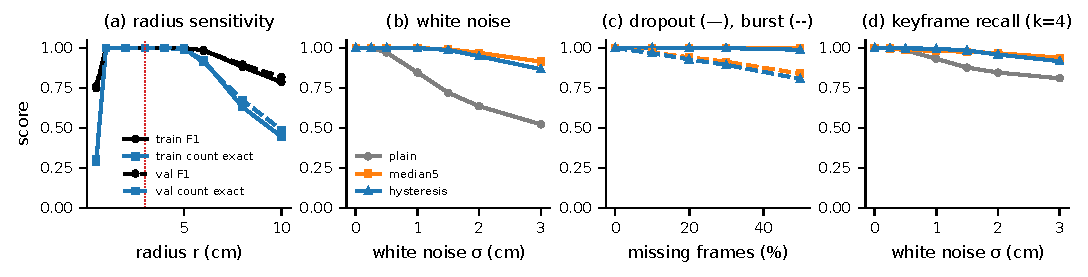
\includegraphics[width=\linewidth]{fig6_event_detection}
\caption{Event detection. (a) F1 and count exact rate versus radius $r$ on training and validation data. (b) F1 versus white-noise level for the plain, median5 and hysteresis detectors. (c) F1 versus the fraction of missing frames, independent (solid) and contiguous (dashed). (d) Recall of K4 memory keyframes ($\pm3$ frames) versus white-noise level.}
\label{fig:events}
\end{figure}

\subsection{What a fixed-budget memory retains (RQ4)}
\label{sec:res_memory}
Table~\ref{tab:coverage} compares memories at the 16-frame budget over 5318 decision points of the validation demonstrations. Figure~\ref{fig:timeline} shows the frames each memory selects in one episode.

\emph{Uniform memory loses picks systematically.} It covers only 57.0\% of the completed picks, and only 43.1\% of decisions can count the picks from memory. Even the most recent pick is covered in only 67.5\% of decisions. A 16-frame uniform memory over a 500-frame episode keeps one frame every 30 frames, while a pick lasts about a dozen frames, so coverage is a matter of chance: random memory reaches 43.2\%, the same order. A recent-frame window is worse still (8.0\%), because it forgets everything before the last 16 frames.

\emph{Forgetting grows with operating time, as the coverage analysis predicts.} Figure~\ref{fig:theory} breaks coverage down by decision time over the 200 validation episodes (7884 decision--pick pairs). At a 16-frame budget, uniform memory covers 97.8\% of completed picks in the first 200 frames, then 56.6\%, 40.8\% and only 26.4\% beyond 600 frames. The most recent pick falls from 97.8\% to 21.7\%: late in an episode, the policy has usually lost sight of the pick it has just made. Equation~(\ref{eq:coverage}) predicts the measured coverage of uniform memory to within 0.012 at every budget (predicted / measured: 0.282 / 0.270 for $B=8$, 0.562 / 0.570 for $B=16$ and 0.882 / 0.883 for $B=32$) and tracks its decay over time (Fig.~\ref{fig:theory}c). The failure is therefore structural, a consequence of sampling geometry, and cannot be tuned away. \pekm\ removes the dependence on time. Both $k=4$ and $k=8$ cover the most recent pick at every decision time (100\%), and $k=8$ covers 94.6\% or more of all completed picks even beyond 600 frames.

\begin{figure}[t]
\centering
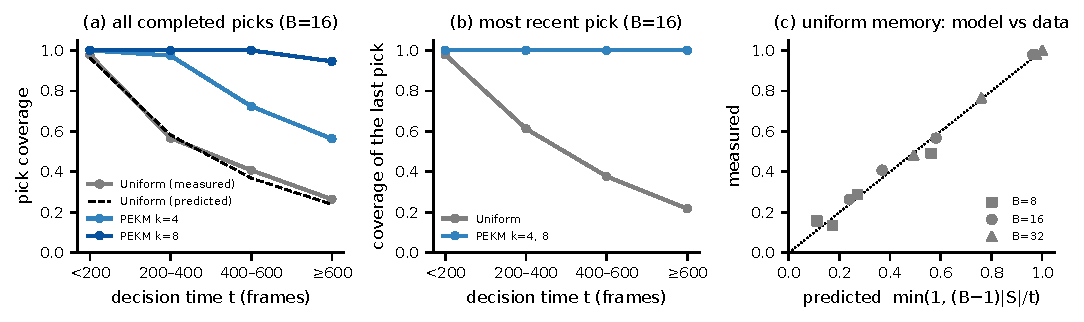
\includegraphics[width=\linewidth]{fig_coverage_theory}
\caption{Time-indexed memory forgets more the longer the robot works. (a) Coverage of all completed picks versus decision time at $B=16$: uniform memory (measured, and predicted by Eq.~(\ref{eq:coverage})) and PEKM. (b) Coverage of the most recent pick. (c) Predicted versus measured coverage of uniform memory for every budget and decision-time bin.}
\label{fig:theory}
\end{figure}

\emph{\pekm\ retains recent picks by construction.} With $k=4$, the last two picks are covered at every decision (100\%), and overall coverage rises to 87.6\%. With $k=8$, coverage reaches 99.6\% and count recoverability 99.2\%, reaching 100\% in FruitOccludedRipe, which has at most three picks. Per task, count recoverability rises from 0.389 (U) to 0.985 (K8) in FruitCount and from 0.485 to 1.000 in FruitOccludedRipe.

\emph{The temporal context is preserved.} The median gap between memory frames grows only from 14 (U) to 17 frames, so the non-event part of the memory keeps nearly the resolution of uniform sampling (Fig.~\ref{fig:coverage}c). The soft variant concentrates more frames near fruits (near-frame fraction 0.265 for $\alpha=1$, six times that of U) and covers older picks evenly. It does so at the cost of the most recent pick (0.814) and of temporal context (median gap 63 frames), which is why hard reservation is the main method.

\emph{Budget efficiency.} Coverage versus budget (Fig.~\ref{fig:coverage}a) shows that K4 with 8 frames (85.9\%) exceeds uniform memory with 16 frames (57.0\%) and approaches uniform memory with 32 frames (88.3\%). K8 with 16 frames (99.6\%) exceeds uniform memory with 32. For field platforms constrained by GPU memory and latency, this means the same event information with a memory two to four times shorter.

\begin{table}[t]
\centering
\caption{Information retained by 16-frame memories (validation, both tasks; 5318 decisions, 7841 decision--pick pairs). Last / 2nd / 3rd: coverage of the most recent, second and third most recent pick. Near: fraction of memory frames with $d_t \le r$. Gap: median gap between memory frames (frames).}
\label{tab:coverage}
\footnotesize
\begin{adjustbox}{max width=\textwidth}\begin{tabular}{lcccccccc}
\toprule
Memory & Event cov. & Run cov. & Count rec. & Last & 2nd & 3rd & Near & Gap\\
\midrule
Uniform (U, K0) & 0.570 & 0.461 & 0.431 & 0.675 & 0.472 & 0.416 & 0.042 & 14\\
Recent & 0.080 & 0.069 & 0.046 & 0.145 & 0.000 & 0.000 & 0.049 & 209\\
Random & 0.432 & 0.364 & 0.329 & 0.533 & 0.351 & 0.231 & 0.040 & 41\\
PEKM $k=2$ & 0.729 & 0.681 & 0.579 & 1.000 & 0.430 & 0.336 & 0.085 & 17\\
\textbf{PEKM $k=4$} & \textbf{0.876} & \textbf{0.875} & \textbf{0.814} & \textbf{1.000} & \textbf{1.000} & 0.136 & 0.110 & 17\\
\textbf{PEKM $k=8$} & \textbf{0.996} & \textbf{0.995} & \textbf{0.992} & \textbf{1.000} & \textbf{1.000} & \textbf{1.000} & 0.123 & 17\\
PEKM $k=12$ & 1.000 & 1.000 & 1.000 & 1.000 & 1.000 & 1.000 & 0.124 & 17\\
PEKM-S $\alpha=0.5$ & 0.878 & 0.854 & 0.756 & 0.811 & 0.982 & 0.948 & 0.153 & 31\\
PEKM-S $\alpha=1$ & 0.897 & 0.873 & 0.770 & 0.814 & 1.000 & 1.000 & 0.265 & 63\\
\bottomrule
\end{tabular}\end{adjustbox}
\end{table}

\begin{figure}[t]
\centering
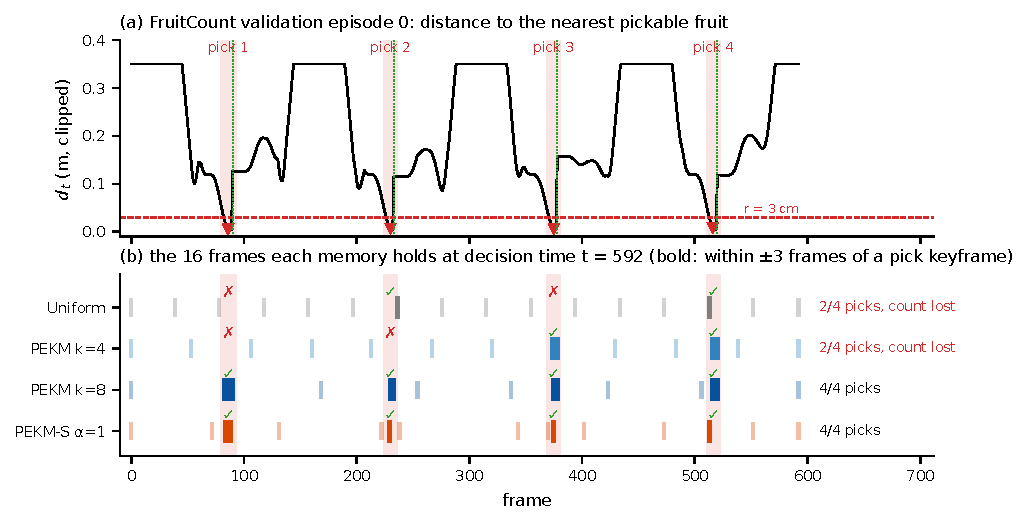
\includegraphics[width=\linewidth]{fig4_memory_timeline}
\caption{Memory timeline of one FruitCount validation episode. Top: the TCP-to-fruit distance $d_t$ with detected events (shaded), contact keyframes (triangles), the radius $r$ (dashed) and fruit detachments (dotted). Bottom: the 16 frames held by uniform memory, PEKM ($k=4$, $k=8$) and PEKM-S ($\alpha=1$) at the last decision.}
\label{fig:timeline}
\end{figure}

\begin{figure}[t]
\centering
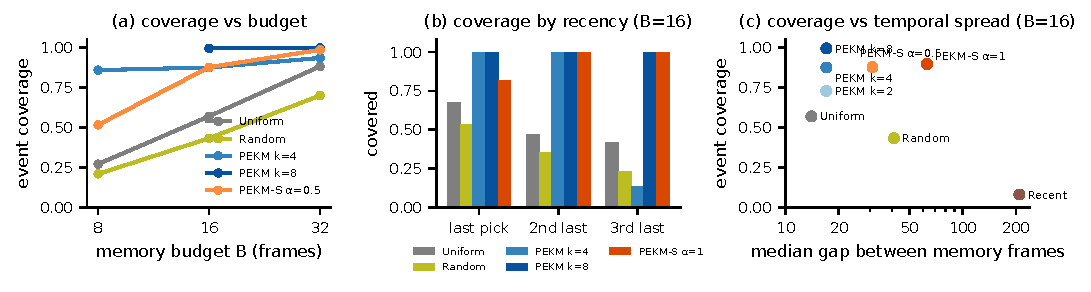
\includegraphics[width=\linewidth]{fig7_memory_coverage}
\caption{Memory coverage. (a) Event coverage versus budget $B$. (b) Coverage of the last three picks at $B=16$. (c) Event coverage versus median gap between memory frames: PEKM raises coverage without sacrificing temporal resolution.}
\label{fig:coverage}
\end{figure}

\subsection{Fruit segmentation with SAM (RQ5)}
\label{sec:res_sam}
Table~\ref{tab:sam} and Fig.~\ref{fig:sam} compare fruit segmentation on 8644 rendered validation images, containing 13{,}424 front-camera and 4877 wrist-camera fruit instances.

\emph{Prompted SAM gives the most accurate masks.} \fdm\ detects fruits with an instance F1 of 0.991 on the front camera and 0.983--0.984 on the wrist camera. Its masks are tighter than those of colour thresholding: the IoU of matched front-camera instances is 0.974--0.978, against 0.945 for HSV. Boundary accuracy matters here because fruit centres are estimated from the back-projected mask (Section~\ref{sec:fdm}), and the resulting anchors are accurate to 0.48~cm (Table~\ref{tab:anchors}). SAM also recovers more partially hidden fruits: front-camera recall is 0.967--0.976 against 0.952 at 25--75\% visibility, and 0.633--0.688 against 0.615 below 25\%. Ripeness is classified correctly for every matched instance by all methods.

\emph{Prompts are essential.} Without prompts, automatic SAM masks filtered by colour and shape (SAM-AUTO) have high precision (0.994--0.996) but miss partially hidden fruits. Front-camera recall drops to 0.57--0.62 at 25--75\% visibility and to 0.21--0.26 below 25\%. SAM-AUTO is also four to seven times slower (395--626~ms per image), because it decodes a dense grid of point prompts.

\emph{A small backbone suffices.} The three backbones have the same F1 (0.991, front camera) and differ by at most 0.004 in IoU, while latency grows from 94~ms (ViT-B) to 195~ms (ViT-L) and 309~ms (ViT-H). The image encoder accounts for more than 90\% of this time. Since anchors are built once per episode and the per-frame vacancy test needs no segmentation (Section~\ref{sec:fdm}), SAM runs once per episode in \fdm, and ViT-B is the practical choice for an embedded platform.

\emph{The remaining gap lies in prompting barely visible fruits.} With ground-truth boxes as prompts, SAM reaches F1 0.999 and a front-camera recall of 0.899 below 25\% visibility. The difference from \fdm\ comes from fruits too small or too occluded to produce a colour component, not from SAM's masks.

\begin{table}[t]
\centering
\caption{Fruit instance segmentation and ripeness on rendered validation images (8644 images; 13{,}424 front and 4877 wrist instances). F1 at IoU $\ge 0.5$. IoU: mean over matched front-camera instances. R (vis.): front-camera recall by visible fraction (418 instances at 25--75\%, 109 below 25\%). Latency: median per front image on one L20 GPU. SAM-AUTO was evaluated on every 5th frame.}
\label{tab:sam}
\footnotesize
\begin{adjustbox}{max width=\textwidth}\begin{tabular}{llccccccc}
\toprule
Method & Backbone & F1 front & F1 wrist & IoU & R (25--75\%) & R ($<$25\%) & Ripeness & ms/img\\
\midrule
HSV thresholds & -- & 0.990 & 0.980 & 0.945 & 0.952 & 0.615 & 1.000 & 1.4\\
SAM-AUTO & ViT-B & 0.937 & 0.983 & 0.979 & 0.573 & 0.263 & 1.000 & 395\\
SAM-AUTO & ViT-H & 0.941 & 0.981 & 0.970 & 0.618 & 0.211 & 1.000 & 626\\
\fdm & ViT-B & \textbf{0.991} & \textbf{0.984} & 0.974 & 0.967 & 0.633 & 1.000 & 94\\
\fdm & ViT-L & \textbf{0.991} & \textbf{0.984} & \textbf{0.978} & \textbf{0.976} & \textbf{0.688} & 1.000 & 195\\
\fdm & ViT-H & \textbf{0.991} & 0.983 & 0.975 & 0.971 & 0.651 & 1.000 & 309\\
\midrule
SAM-GTBOX (upper bound) & ViT-H & 0.999 & 0.999 & 0.980 & 1.000 & 0.899 & 1.000 & --\\
\bottomrule
\end{tabular}\end{adjustbox}
\end{table}

\begin{figure}[t]
\centering
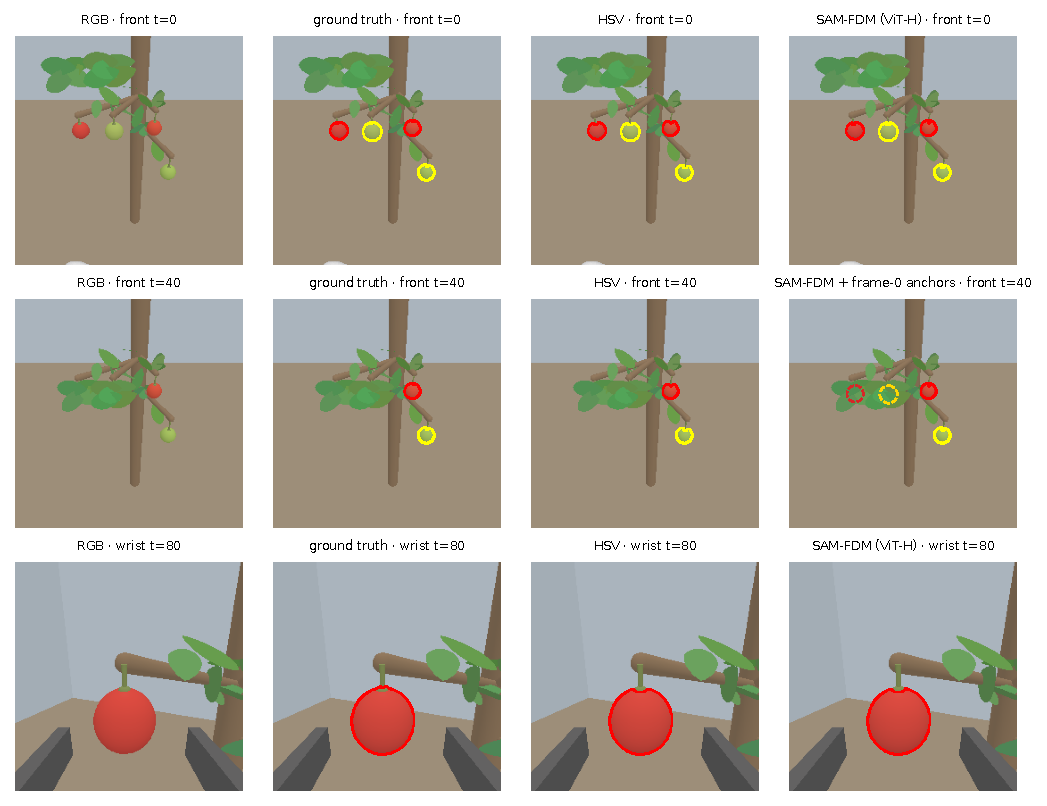
\includegraphics[width=\linewidth]{fig8a_sam_qualitative}\\[2pt]
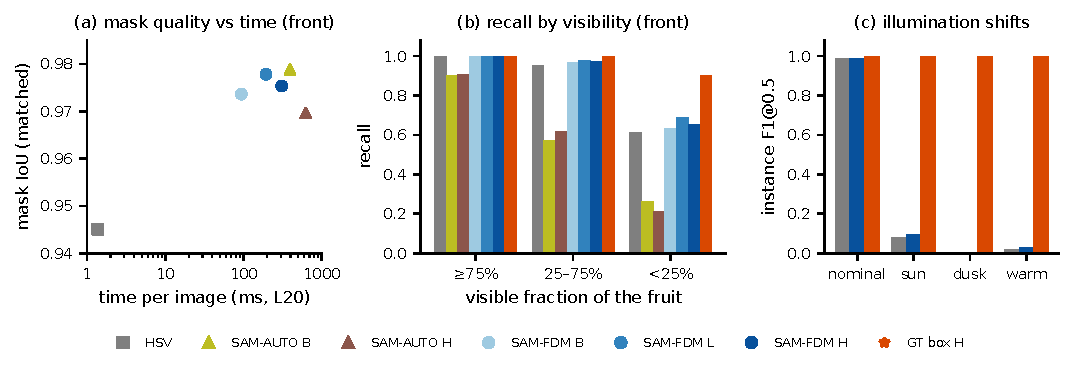
\includegraphics[width=\linewidth]{fig8b_sam_quantitative}
\caption{Fruit segmentation. Top: a FruitOccludedRipe validation episode before the gust (front, $t=0$), after it (front, $t=40$) and at contact (wrist, $t=80$). Columns show the image, ground truth, HSV thresholds and \fdm\ (ViT-H); red contours mark ripe fruits and yellow contours unripe ones. At $t=40$, dashed circles are the frame-0 anchors, which keep the two leaf-hidden fruits in memory. Bottom: (a) mask IoU versus latency; (b) front-camera recall by visible fraction; (c) F1 under illumination shifts.}
\label{fig:sam}
\end{figure}

\emph{Illumination.} To anticipate field conditions, we re-rendered every third frame with three photometric shifts: overcast or dusk ($0.55\,x^{1.2}$), direct sun ($1.35\,x^{0.85}$) and a warm low sun (channel gains 1.12 / 1.00 / 0.80). Colour thresholds were kept as calibrated (Table~\ref{tab:light}). SAM's masks are invariant to these changes: given correct box prompts, F1 stays at 0.999 and IoU at 0.979 under all three conditions. Fixed colour thresholds, by contrast, do not transfer outside their calibration conditions. Their F1 falls below 0.1, and \fdm\ inherits this through its prompts. The analysis locates precisely which component must adapt for field use: the prompt generator. Because prompts are the only input that \fdm\ takes from colour, the thresholds can be replaced by an illumination-normalized colour model or a learned fruit detector without changing SAM, the anchors or the policy. \tbd{Optional: add a row with colour normalization (grey-world white balance + brightness normalization) before thresholding, or a detector trained on randomized-lighting renders, as prompt source.}

\begin{table}[t]
\centering
\caption{Segmentation F1 under illumination shifts (front and wrist cameras together; 6396 instances per shifted condition, 18{,}301 nominal). Colour thresholds as calibrated under nominal lighting. SAM backbone ViT-H.}
\label{tab:light}
\small
\begin{adjustbox}{max width=\textwidth}\begin{tabular}{lcccc}
\toprule
Condition & HSV thresholds & \fdm\ (colour prompts) & SAM-GTBOX F1 & SAM-GTBOX IoU\\
\midrule
Nominal & 0.987 & 0.989 & 0.999 & 0.979\\
Direct sun (bright) & 0.079 & 0.096 & 0.999 & 0.979\\
Overcast / dusk (dark) & 0.000 & 0.000 & 0.999 & 0.979\\
Low sun (warm) & 0.018 & 0.031 & 0.999 & 0.979\\
\bottomrule
\end{tabular}\end{adjustbox}
\end{table}

\subsection{From RGB-D images to event memory (RQ6)}
\label{sec:res_chain}
Tables~\ref{tab:anchors} and~\ref{tab:chain} evaluate the complete chain on the 199 validation episodes. It uses only the recorded front RGB-D frames, forward kinematics and the gripper state, with no simulator ground truth.

\emph{Anchors.} Frame-0 anchors recover 99.8\% of fruits with 99.5\% precision. The median localization error is 0.48~cm (90th percentile 0.58~cm), below a fifth of the fruit radius, and ripeness is classified without error. All 138 ripe fruits that the gust later hides behind leaves have an anchor.

\emph{Distance, events and memory.} The perceived distance $\hat d_t$ has a median error of 0.34~cm in the near range (90th percentile 0.48~cm), well inside the accuracy specification derived in Section~\ref{sec:res_robust}. Events detected from $\hat d_t$ match the ground truth exactly: precision, recall and F1 are 1.000, the count is exact in every episode, the contact lead is 4 frames as with ground truth, and the release error is 0 frames. The resulting PEKM memories recover every ground-truth keyframe (keyframe recall 1.000). The Jaccard similarity is 0.948 for $k=4$ and 0.941 for $k=8$. The remaining differences come from contact frames shifting by one or two frames, which moves the uniform part of the memory; no event information is lost. Consumer-grade depth noise leaves all results unchanged.

\emph{Spatial memory before occlusion is necessary.} When anchors are built after the gust (frame 29), anchor recall drops to 0.783, and to 0.568 in FruitOccludedRipe. None of the 138 leaf-hidden ripe fruits receives an anchor. Event recall in FruitOccludedRipe falls to 0.450, and \emph{no} FruitOccludedRipe episode has the correct pick count (0.00, against 1.00 with frame-0 anchors). FruitCount, which has no foliage occlusion, is unaffected. Perceiving a fruit while it is visible and remembering where it is is therefore a precondition for remembering that it was picked.

\emph{Grasp evidence closes the visual blind spot.} With depth vacancy alone, the arm and the carried fruit occlude the anchor's pixels during carrying, so detachment is confirmed only after the arm leaves: the release keyframe is late by a median of 16 frames, and the memory Jaccard drops to 0.685. Adding the gripper-holding cue, a proprioceptive signal available at almost no cost, removes the delay.

\emph{Anchors are more reliable than per-frame detection.} Without anchors, the fruit being carried in the gripper is still detected as the nearest fruit. The release error grows to 52 frames, and spurious events appear (precision 0.821, count exact in 62\% of episodes; 0.759 and 46\% in FruitCount, where carried fruits repeatedly disappear and reappear). Hysteresis suppresses some of them (precision 0.942), but the memory Jaccard remains 0.421. Figure~\ref{fig:chain} illustrates these behaviours on one episode.

\begin{table}[t]
\centering
\caption{Fruit anchors from \fdm\ (ViT-H) on 199 validation episodes, matched to the true fruit positions at frame 0 (5 cm gate). Hidden ripe: fraction of ripe fruits later hidden by leaves that have an anchor ($n=138$).}
\label{tab:anchors}
\small
\begin{adjustbox}{max width=\textwidth}\begin{tabular}{lccccc}
\toprule
Anchors & Recall & Precision & Error med / p90 (cm) & Ripeness acc. & Hidden ripe\\
\midrule
Frame 0 (before gust, ours) & 0.998 & 0.995 & 0.48 / 0.58 & 1.000 & \textbf{1.000}\\
Frame 0 + depth noise & 0.998 & 0.995 & 0.45 / 0.56 & 1.000 & 1.000\\
Frame 29 (after gust) & 0.783 & 0.993 & 0.49 / 0.58 & 1.000 & 0.000\\
\bottomrule
\end{tabular}\end{adjustbox}
\end{table}

\begin{table}[t]
\centering
\caption{Events and memory from perceived distances (199 validation episodes; plain detector, hysteresis in parentheses). Dist.\ err.: median / 90th-percentile error of $\hat d_t$ where $d_t \le 10$ cm. Rel.\ err.: median error of the release keyframe (frames). Jaccard and KF recall: agreement of the K4 memory with the memory computed from ground truth. For K8, Jaccard is 0.941 / 0.941 / 0.660 / 0.730 / 0.363 and KF recall 1.000 / 1.000 / 0.847 / 0.882 / 0.782 for the rows below GT.}
\label{tab:chain}
\footnotesize
\begin{adjustbox}{max width=\textwidth}\begin{tabular}{lcccccccc}
\toprule
Distance source & Dist.\ err.\ (cm) & P & R & F1 & Count & Rel.\ err. & Jaccard & KF recall\\
\midrule
GT (upper bound) & 0 / 0 & 1.000 & 1.000 & 1.000 & 1.00 & 0 & 1.000 & 1.000\\
\textbf{\fdm\ (ours)} & \textbf{0.34 / 0.48} & \textbf{1.000} & \textbf{1.000} & \textbf{1.000} & \textbf{1.00} & \textbf{0} & \textbf{0.948} & \textbf{1.000}\\
\fdm\ + depth noise & 0.31 / 0.46 & 1.000 & 1.000 & 1.000 & 1.00 & 0 & 0.948 & 1.000\\
Depth-only & 0.39 / 10.76 & 1.000 & 1.000 & 1.000 & 1.00 & 16 & 0.685 & 0.845\\
Post-gust anchors & 0.39 / -- & 1.000 & 0.743 & 0.853 & 0.50 & 0 & 0.741 & 0.880\\
Per-frame & 0.39 / 12.79 & 0.821 (0.942) & 1.000 & 0.902 (0.970) & 0.62 (0.85) & 52 & 0.421 & 0.755\\
\bottomrule
\end{tabular}\end{adjustbox}
\end{table}

\begin{figure}[t]
\centering
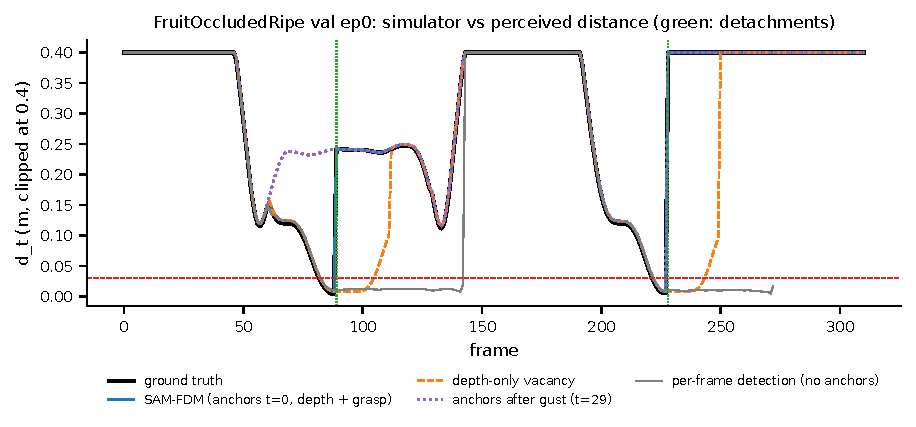
\includegraphics[width=\linewidth]{fig_e6_perceived_distance}
\caption{Perceived versus ground-truth distance in one FruitOccludedRipe episode. Vertical lines mark fruit detachments. \fdm\ follows the ground truth. Depth-only vacancy confirms detachment late, post-gust anchors miss the hidden ripe fruit, and per-frame detection tracks the carried fruit.}
\label{fig:chain}
\end{figure}

\subsection{Closed-loop harvesting (RQ7)}
\label{sec:res_closed}
Table~\ref{tab:closed} reports closed-loop results on validation episodes 50--99 (150 trials per task and condition). \tbd{Main results text after the sealed evaluation: success rates of K0/K4/K8 per task with paired differences, 95\% CIs and Holm-adjusted p-values; process metrics (completion, over-pick in FruitCount, wrong-pick in FruitOccludedRipe, drops, steps); stratification by quota $N$ (2 / 3 / 4--5); validity gates (engineering errors, frame-selection audit).}

\begin{table}[t]
\centering
\caption{Closed-loop harvesting on validation episodes 50--99 (3 seeds; 150 trials per cell). Paired differences with 95\% bootstrap CIs; Holm-adjusted p-values over the primary family.}
\label{tab:closed}
\footnotesize
\begin{adjustbox}{max width=\textwidth}\begin{tabular}{llcccccc}
\toprule
Task & Memory & Success & Completion & Over-/wrong-pick & Drop & Steps & $\Delta$ vs K0 [95\% CI]\\
\midrule
FruitCount & K0 (uniform) & \tbd{} & \tbd{} & \tbd{} & \tbd{} & \tbd{} & --\\
 & K4 (PEKM) & \tbd{} & \tbd{} & \tbd{} & \tbd{} & \tbd{} & \tbd{}\\
 & K8 (PEKM) & \tbd{} & \tbd{} & \tbd{} & \tbd{} & \tbd{} & \tbd{}\\
FruitOccludedRipe & K0 (uniform) & \tbd{} & \tbd{} & \tbd{} & \tbd{} & \tbd{} & --\\
 & K4 (PEKM) & \tbd{} & \tbd{} & \tbd{} & \tbd{} & \tbd{} & \tbd{}\\
 & K8 (PEKM) & \tbd{} & \tbd{} & \tbd{} & \tbd{} & \tbd{} & \tbd{}\\
\bottomrule
\end{tabular}\end{adjustbox}
\end{table}

\subsection{Ablations and counterfactual controls}
\label{sec:res_ablation}
Table~\ref{tab:ablation} lists the test-time ablations, evaluated with the K4 policy under the same paired protocol. \tbd{Results text: (a) keyframe cap; (b) budget; (c) radius 1/3/5 cm; (d) hard vs soft selection; (e) signal source GT / SAM-FDM / noisy GT; (f) counterfactual controls EVU, EVR and EVA; (g) keyframe composition (contact only / release only / both).}

\begin{table}[t]
\centering
\caption{Ablations (test-time variants of the K4 policy unless noted; paired differences to the default configuration).}
\label{tab:ablation}
\footnotesize
\begin{adjustbox}{max width=\textwidth}\begin{tabular}{llcc}
\toprule
Factor & Setting & FruitCount $\Delta$ & FruitOccludedRipe $\Delta$\\
\midrule
Keyframe cap $k$ (trained) & 0 / 4 / 8 & \tbd{} & \tbd{}\\
Radius $r$ & 1 / 3 / 5 cm & \tbd{} & \tbd{}\\
Selection & hard (PEKM) / soft (PEKM-S, $\alpha=0.5$) & \tbd{} & \tbd{}\\
Signal source & GT / \fdm\ / GT + 1 cm noise & \tbd{} & \tbd{}\\
Counterfactual & EV / EVU / EVR / EVA & \tbd{} & \tbd{}\\
Keyframes & contact / release / both & \tbd{} & \tbd{}\\
Training data & clean (C0) / clean + DART-H (K0) & \tbd{} & \tbd{}\\
\bottomrule
\end{tabular}\end{adjustbox}
\end{table}

\subsection{Open-loop accuracy, closed-loop drift and DART-H (RQ8)}
\label{sec:res_dart}
Table~\ref{tab:openloop} evaluates a policy trained on clean demonstrations in open loop, predicting actions at the demonstrated states. TCP errors at the end of a 16-step chunk are 1.7--2.4~cm (median), and 0.7--1.1~cm during the near-fruit phase, an order of magnitude below the motion within a chunk (about 10~cm). The gripper open/close direction agrees with the demonstration in 98--99.5\% of decisions. Training and validation errors are nearly identical: the policy has learned the demonstrations and generalizes to unseen layouts. In closed loop, however, small deviations accumulate and move the robot into states that clean demonstrations do not cover. This is the covariate shift that DART-H targets. Its perturbations (median TCP displacement 2.5~cm) match the scale of these errors. \tbd{Closed-loop C0 vs K0 comparison and the time of first departure from the demonstrated distribution.}

\begin{table}[t]
\centering
\caption{Open-loop (teacher-forced) accuracy of a uniform-memory policy trained on clean demonstrations (10 episodes per set). TCP error at horizons 1, 8 and 16 of the action chunk; near: horizon 16 while $d_t \le 10$ cm.}
\label{tab:openloop}
\small
\begin{adjustbox}{max width=\textwidth}\begin{tabular}{llccc}
\toprule
Set & Task & TCP error h1 / h8 / h16 (cm) & Near h16 (cm) & Gripper agreement\\
\midrule
Train & FruitCount & 0.44 / 1.23 / 1.83 & 0.75 & 99.5\%\\
Train & FruitOccludedRipe & 0.42 / 1.25 / 1.66 & 0.70 & 99.2\%\\
Validation & FruitCount & 0.51 / 1.37 / 2.38 & 1.14 & 98.0\%\\
Validation & FruitOccludedRipe & 0.40 / 1.32 / 1.75 & 0.78 & 98.9\%\\
\bottomrule
\end{tabular}\end{adjustbox}
\end{table}

\subsection{Memory content matters for VLA policies}
\label{sec:res_general}
To show that the frames a VLA policy remembers affect its actions, and not only an offline coverage metric, we evaluated the base policy on a general manipulation-memory benchmark (\tbd{cite RoboMME}) under sealed protocols (Table~\ref{tab:general}). Removing the history memory collapses success on a pattern-recall task from 66.7\% to 1.7\%. Halving the budget from 32 to 16 frames reduces it from 64.4\% to 26.7\%. Replacing a single memory slot changes the expert's action loss consistently: the ranking of slots is reproducible with a reliability of 0.97--0.99 across four tasks. Within a fixed budget, the choice of frames therefore has a substantial effect on the policy. This is the premise of \pekm.

\begin{table}[t]
\centering
\caption{Memory ablations of the base VLA on a general manipulation-memory benchmark (paired bootstrap, Holm-adjusted).}
\label{tab:general}
\footnotesize
\begin{adjustbox}{max width=\textwidth}\begin{tabular}{p{4.6cm}p{7.6cm}}
\toprule
Intervention & Result\\
\midrule
No history memory (pattern-recall task) & 66.7\% $\rightarrow$ 1.7\% ($-65.0$ pp, 95\% CI [$-81.7$, $-46.7$], $p<0.001$)\\
No memory (video-swap task) & $-11.7$ pp (95\% CI [$-20.0$, $-3.3$], $p=0.006$)\\
Budget 32 $\rightarrow$ 16 frames (pattern recall) & 64.4\% $\rightarrow$ 26.7\% ($-37.8$ pp, $p<0.001$)\\
Single-slot replacement (counterfactual action loss) & Slot ranking reliability 0.97--0.99 over four tasks; cross-fitted relative gain 2.5--12.4\%\\
\bottomrule
\end{tabular}\end{adjustbox}
\end{table}

\subsection{Run-time cost}
\label{sec:res_cost}
\pekm\ adds negligible computation. At $t=1000$ frames, one selection takes 117~$\mu$s (median; 99th percentile 125~$\mu$s) on a CPU core, against 39~$\mu$s for uniform sampling, which is negligible compared with one VLA inference (\tbd{VLA inference latency, ms}). Because the budget is unchanged, the memory footprint and inference cost of the policy are identical to the uniform baseline. \fdm\ segments an image in 94 / 195 / 309~ms with ViT-B / ViT-L / ViT-H on one L20 GPU, dominated by the image encoder. It runs SAM only when anchors are built, once per episode. The per-frame work, projecting a handful of anchors and reading their depth and the gripper state, takes well under a millisecond.

\section{Discussion}
\label{sec:discussion}

\subsection{From time-indexed to event-indexed memory}
The central lesson of this work is that the memory of an embodied agricultural agent should be organized around what happens, not around when it happens. The coverage analysis and its close agreement with measurement (Fig.~\ref{fig:theory}) show that the failure of uniform memory is structural. For any fixed budget, the fraction of interaction events that time-indexed memory retains vanishes as operation lengthens. This is precisely the regime of practical harvesting, in which a robot works continuously along a row rather than in short, isolated episodes. Enlarging the budget only postpones the problem, at a cost that grows quadratically. Event indexing removes the dependence on operating time altogether. Picks are short (about a dozen frames out of several hundred) but physically unambiguous: event detection is exact over a 1--4~cm plateau of the radius, set by fruit size rather than tuned. Reserving two slots per remembered pick makes the memory complete for the information the task needs (99.6\% of picks) at no cost in budget, latency or architecture.

The approach--act--leave structure is not specific to fruit picking. Pruning cuts, fruit thinning, flower pollination and spot spraying all consist of discrete interactions with plant organs. For each of them, the distance from the tool to the nearest organ still to be treated is an equally natural event signal, and the radius scales with organ size. We therefore expect event-centric memory to transfer to these operations with only a redefinition of the target set $\mathcal{P}_t$. It could serve as a general memory principle for agricultural manipulation, beyond the harvesting tasks studied here.

\subsection{Designing perception for memory}
The perception experiments yield two lessons for agricultural perception systems that feed a learned policy.

First, \emph{what perception must deliver is a specification, not a maximum}. Event-based memory tolerates up to about 1.5~cm of white noise or 2~cm of correlated noise in the distance signal, together with arbitrary independent dropouts and centimetre-level bias. \fdm\ is an order of magnitude more accurate than this specification (0.34~cm median error), and remains so under consumer-grade depth noise. This margin indicates that a cheaper detector or sensor can be substituted, and the scalar interface makes such substitution straightforward.

Second, \emph{memory starts with perception}. Leaf-hidden ripe fruits are recoverable only if they were anchored while visible. Without that spatial memory, no occluded-task episode is counted correctly. In practice this argues for a deliberate observation phase, or for anchoring fruits whenever they become visible during operation, as well as for redundant evidence of picking. The gripper-holding cue removed a 16-frame delay at essentially zero cost, so proprioceptive and tactile signals should be treated as perception inputs for event detection, not only as control feedback. Explicit anchors (geometric memory) and \pekm\ (visual memory of events) thus play complementary roles. Anchors remember \emph{where} fruits are, and the event memory lets the policy see \emph{what happened} to them.

\subsection{Compounding errors in end-to-end harvesting}
End-to-end policies are accurate in open loop: about 2~cm TCP error at the end of a chunk, and 98--99.5\% agreement on gripper actions. Accuracy at the demonstrated states, however, does not guarantee success in closed loop, where small deviations accumulate into states that clean demonstrations do not cover. For harvesting, where the gripper must enclose a 5-cm fruit, a few centimetres of drift is the difference between a grasp and a miss. Recovery data that covers this drift, generated without an expert in the loop and restricted to the phases where it is safe, addresses the data rather than the model. \tbd{Discussion of the closed-loop DART-H and PEKM results once available.}

\subsection{Practical implications}
For field robots, which run on embedded GPUs with tight memory and latency budgets, the budget efficiency of event memory matters directly. With \pekm, an 8-frame memory retains more pick information than a 16-frame uniform one, and a 16-frame memory more than a 32-frame one, at a selection cost of about 0.1~ms. Because the selection is a pure function of a logged scalar signal, every memory the policy saw can be reproduced and audited after the fact. This property is useful for diagnosing failures in the field and supports the transparency expected of autonomous agricultural machines.

\subsection{Towards memory-aware agricultural foundation models}
As vision--language--action and other foundation models enter agricultural robotics, the question of what such models remember will become as important as what they perceive. Agricultural tasks are long, repetitive and partially observable, and their success depends on a running account of the plants already treated, the fruits still hidden and the quota still open. HarvestMem shows that this account can be supplied without changing the model's architecture or adding parameters. A physically grounded event signal, a spatial memory of objects acquired while they are visible, and a parameter-free selection rule turn a generic memory-augmented policy into one that remembers what matters for the task. We view this decoupling as a practical path for adapting general-purpose robot foundation models to agriculture. The agricultural knowledge is encoded in \emph{what counts as an event}, which domain experts can specify and audit, rather than in additional network parameters.

\subsection{Limitations}
This study has several limitations.
\begin{itemize}
\item \textbf{Simulation.} The study is conducted in simulation. Fruits are rigid spheres; stems detach after a fixed holding time, and branch mechanics are simplified. Wind acts only during the observation phase, and fruits do not swing.
\item \textbf{Perception scope.} Colour prompts suffice for red and green fruits on a rendered canopy under the calibrated lighting, but fixed thresholds do not transfer to strongly different illumination (Table~\ref{tab:light}), even though SAM's masks do. Green fruits against green foliage, natural illumination and clustered fruits (e.g.\ tomato trusses or grapes) will require learned or illumination-normalized prompt generators, and an event definition for clusters.
\item \textbf{Robot and scene diversity.} One tree type and one arm were used for closed-loop evaluation, although the generator also supports a 6-DoF arm.
\item \textbf{Real-world validation.} Transfer to a real orchard has not been tested yet. A RealMan RM75-B with an EG2 gripper and an RGB-D camera, matching the simulated system, is the planned platform.
\end{itemize}
\tbd{Add any limitation revealed by the closed-loop results.}

\subsection{Future work}
Several extensions follow directly from the framework:
\begin{enumerate}
\item The event detector already counts picks, and this count can be given to the policy as a short text prompt (e.g.\ ``picked 2 of 3''), giving an explicit symbolic memory alongside the visual one.
\item A lightweight learned memory manager could be trained from counterfactual action-loss signals and compared with the rule-based selection.
\item Anchors of hidden ripe fruits could guide active leaf pushing before the approach.
\item Wind can be extended to the whole episode with swinging fruits.
\item Sim-to-real transfer with domain randomization of illumination, fruit colour and foliage density.
\end{enumerate}

\section{Conclusions}
\label{sec:conclusions}

Selective harvesting robots must act on what they can no longer see: fruits hidden by foliage and picks whose results are out of view. This paper showed that the time-indexed memory of current vision--language--action policies is structurally unsuited to this requirement, because its coverage of interaction events decays with operating time. We proposed HarvestMem, an event-centric alternative. It couples a spatial memory of 3D fruit anchors, acquired by promptable segmentation while fruits are visible, with an episodic memory that reserves the contact and detachment keyframes of picks in the policy's fixed memory budget. The main findings are:
\begin{enumerate}
\item The coverage of completed picks by uniform memory follows a simple sampling law, $c_U(t) \approx \min(1, (B-1)|S|/t)$, which predicts the measured coverage to within 0.012. At a 16-frame budget, coverage of the most recent pick falls from 97.8\% early in an episode to 21.7\% after 600 frames.
\item Picking events can be detected exactly from the end-effector-to-fruit distance over a 1--4~cm range of the radius, on clean and perturbed demonstrations alike.
\item Picking-Event Keyframe Memory retains 99.6\% of completed picks against 57.0\% for uniform memory at the same budget, and keeps the most recent pick at every decision time. With 8 frames it outperforms uniform memory with 16, without additional parameters, tokens or inference cost.
\item Using only RGB-D images and proprioception, the SAM-based fruit distance module localizes fruits to 0.48~cm, recovers every leaf-hidden ripe fruit and reproduces the ground-truth picking events exactly. Without spatial memory acquired before occlusion, no occluded-task episode is counted correctly. Spatial memory is thus a precondition for episodic memory in occluded canopies.
\item Event memory tolerates distance errors of up to 1.5--2~cm, dropouts and bias, which gives perception modules an explicit accuracy specification. Promptable SAM gives the most accurate fruit masks (instance F1 0.991, IoU 0.974 with ViT-B at 94~ms per image), and the prompt generator is the component to adapt to field illumination.
\item \tbd{One sentence on closed-loop success with PEKM and DART-H (E7--E9).}
\end{enumerate}
By moving agricultural knowledge into the definition of events rather than into network parameters, HarvestMem offers a principled, auditable way to adapt general-purpose robot foundation models to the long, partially observable operations of agriculture. Validation on a real harvesting robot and extension to pruning, thinning and pollination are the next steps.


\section*{CRediT authorship contribution statement}
\tbd{Conceptualization, Methodology, Software, Validation, Formal analysis, Investigation, Data curation, Writing -- original draft, Writing -- review \& editing, Visualization, Supervision, Funding acquisition.}

\section*{Declaration of competing interest}
The authors declare that they have no known competing financial interests or personal relationships that could have appeared to influence the work reported in this paper.

\section*{Data availability}
The HarvestMem-Sim generator, the demonstration datasets, the evaluation protocols (sealed before the formal runs, with their SHA-256 digests), the analysis scripts and the raw per-episode results will be released at \tbd{repository URL} upon publication.

\section*{Acknowledgements}
\tbd{Funding sources and grant numbers.}

\bibliographystyle{elsarticle-harv}
\bibliography{references}

\end{document}
